% ==============================================================================
% ==============================================================================
%
%      CHOOSE ONE OPTION BY COMMENTING/NOT COMMENTING THE EACH CASE
%
% ==============================================================================
% ==============================================================================

% OPTION 1: Manuscript

% \documentclass[12pt]{article}
%\usepackage{myreviewpckg}

% OPTION 2: Annotated Manuscript

%\documentclass[12pt]{article}
%\usepackage[review]{myreviewpckg}

% OPTION 3: Paper

\documentclass[twocolumn,twoside]{article}
%\usepackage{myreviewpckg}



% ==============================================================================
% ==============================================================================
%
%                      DO NOT MODIFY BEYOND THIS POINT
%
% ==============================================================================
% ==============================================================================

\usepackage{tocloft}
\usepackage{simplemargins}
\usepackage[center,small]{titlesec}
\usepackage{caption}
\usepackage[]{subfig}
\usepackage[round,authoryear,semicolon]{natbib}
\usepackage{setspace}
\usepackage{color}
\usepackage{amsmath}
\usepackage{ifthen}
\usepackage{indentfirst}
\usepackage{balance}
\usepackage[runin]{abstract}
\usepackage{textcomp}
\usepackage{times}
\usepackage{mathptmx}
\usepackage{rotating}
\usepackage{pslatex}
\usepackage{authblk}
\usepackage{datetime}
%\usepackage{multirow}

\usdate

\usepackage{ifpdf}
\ifpdf
	\usepackage[pdftex,bookmarks=false]{hyperref}
\else
	\usepackage{graphics}
	\usepackage{graphicx}
	\usepackage{epsfig}
	\usepackage[dvipdfm,bookmarks=false]{hyperref}
\fi

\clubpenalty=10000  % Orphan - First of paragraph left behind
\widowpenalty=10000 % Widow  - Last of paragraph sent ahead

%\raggedbottom

\captionsetup{font=small,labelfont=bf}
\captionsetup[table]{font=small,labelfont=large}
\captionsetup[subfloat]{font=footnotesize,textfont=scriptsize}

\makeatletter
\if@twocolumn
    \usepackage{fancyhdr}
	\setlength{\parindent}{1.5em}
	\singlespacing
	\setlength{\columnsep}{0.23in}
\else
%    \usepackage[left,pagewise]{lineno}
    \usepackage[left]{lineno}
	\doublespacing
	\captionsetup{font=doublespacing}
	\cftpagenumbersoff{figure}
	\usepackage[tablesfirst,notablist]{endfloat}
	\AtBeginDelayedFloats{\renewcommand\baselinestretch{1.4}}
	\renewcommand\cftloftitlefont{\large}
	\renewcommand\listfigurename{
		\begin{center}
		Figure Captions
		\end{center}
	}
	\setlength{\cftparskip}{2ex}
	\renewcommand\cftfigpresnum{\bf Figure~}
	\renewcommand\cftfigaftersnum{.}
	\renewcommand\cftfignumwidth{5.5em}
\fi
\makeatother

\hypersetup{
    pdfpagelayout=OneColumn,
	colorlinks = true,
	urlcolor   = blue,
	citecolor  = blue,
	linkcolor  = blue
}

\urlstyle{same}

\settopmargin{0.84in}
\setleftmargin{0.8in}
\setrightmargin{0.8in}
\setbottommargin{0.9in}


% Column and figure exceptions
% ----------------------------

\makeatletter
\if@twocolumn
\newcommand\mycolumnwidth{\columnwidth}
\else
\newcommand\mycolumnwidth{0.484\textwidth}
\fi
\makeatother

\makeatletter
\if@twocolumn
\newcommand\mycolumnwidthreduced{0.9\columnwidth}
\else
\newcommand\mycolumnwidthreduced{0.436\textwidth}
\fi
\makeatother

% Some abstract options
% ---------------------

\makeatletter
\if@twocolumn
\setlength{\absleftindent}{0.9in}
\setlength{\absrightindent}{0.9in}
\setlength{\absparindent}{0pt}
\setlength{\abstitleskip}{-1.5em}
\renewcommand\abstracttextfont{\normalsize}
\renewcommand\abstractnamefont{\Large}
%\abslabeldelim{\quad}
\else
\@bsruninfalse
\renewcommand\abstracttextfont{\normalsize}
\renewcommand\abstractnamefont{\large}
\fi
\makeatother

% Title and sections fonts and style
% ----------------------------------

\titleformat{\section}{\centering}{}{0pt}{\large}

\titleformat{\subsection}{}{}{1.5em}{\normalsize}

\titleformat{\subsubsection}[runin]{}{}{0pt}{\normalsize\itshape}[.]


% Manuscript tricks
% -----------------

\newcommand\manuscriptadjust{
\makeatletter
\ifthenelse{\boolean{@twocolumn}}{}{\clearpage}
\makeatother
}

\newcommand\preprintadjust{
\makeatletter
\ifthenelse{\boolean{@twocolumn}}{\small}{}
\makeatother
}

% Figure and Table captions configuration
% ---------------------------------------

\captionsetup[table]{
%	labelfont=large,
	labelsep=newline,
	justification=centerlast,
	textfont=small
}
\captionsetup[figure]{
	labelfont=bf,
	labelsep=period,
	textfont=small
}

\newcommand\introduction{
\makeatletter
\ifthenelse{\boolean{@twocolumn}}{
	~\newline
	\vspace{-15ex}
	\section{Introduction}
	}{
	\section{Introduction}
	}
\makeatother
}

\newcommand\corresponding{%
	\makeatletter\ifthenelse{\boolean{@twocolumn}}
	{}{\thanks{Corresponding author.}~}
\makeatother
}%

\newcommand{\vsmin}{$V_{S_{\min}}$}
\newcommand{\vsmineq}[1]{$V_{S_{\min}}=#1$~m/s}
\newcommand{\vsthirty}{$V_{S30}$}
\newcommand{\vs}{$V_{S}$}
\newcommand{\vseq}[1]{$V_{S}=#1$~m/s}

\newcommand{\vp}{$V_{P}$}
\newcommand{\vpeq}[1]{$V_{P}=#1$~m/s}

\newcommand{\qp}{$Q_{P}$}
\newcommand{\qs}{$Q_{S}$}

\newcommand{\fleq}[1]{$f\leq#1$~Hz}

\newcommand{\fmax}{$f_{_{\max}}$}
\newcommand{\fmaxeq}[1]{$f_{_{\max}}=#1$~Hz}

\newcommand{\eqmag}[1]{$M_{#1}$}

\newcommand{\adomain}[3]{#1~#3 $\times$ #2~#3}
\newcommand{\vdomain}[4]{#1~#4 $\times$ #2~#4 $\times$ #3~#4}


\newcommand{\kmeans}{$k$-$means$}
\newcommand{\feq}[2]{$f = #1-#2$~Hz}


\title{
	\LARGE
	Prioritizing Ground Motion Validation Metrics using Semi-supervised and Supervised Learning
}

\makeatletter
\ifthenelse{\boolean{@twocolumn}}{
\date{}}{}
\makeatother

\makeatletter
\ifthenelse{\boolean{@twocolumn}}{%
\author{by Naeem Khoshnevis and Ricardo Taborda}
}{%
\author[1]{Naeem Khoshnevis}
\author[2,*]{Ricardo Taborda}
\affil[1]{%
	Center for Earthquake Research and Information\\
	The University of Memphis\\
	3890 Central Ave.\\
	Memphis, TN 38152\\
	Email: nkhshnvs@memphis.edu%
}
\affil[2]{%
	Department of Civil Engineering, and
	Center for Earthquake Research and Information\\
	The University of Memphis\\
	3890 Central Ave.\\
	Memphis, TN 38152\\
	Email: ricardo.taborda@memphis.edu%
}
\affil[*]{Corresponding author.}
}
\makeatother



\begin{document}

%\makeatletter
%\if@isreview
%    \input{review-control}
%\fi
%\makeatother


\makeatletter
\if@twocolumn
	\renewcommand\abstractname{\Large Abstract~}
	\twocolumn[
		\vspace{-2em}%
		\maketitle
		\vspace{-2em}%
		\begin{onecolabstract}%
		% 
The validation of ground motion synthetics has received increased attention over the last few years due to the advances in physics-based deterministic and hybrid simulation methods. Unlike for low frequency simulations $(f \le 0.5 Hz)$, for which it has become reasonable to expect a good match between synthetics and data, in the case of high-frequency simulations $(1 Hz \le f)$ it is not possible to match results on a wiggle-by-wiggle basis. This is mostly due to the various complexities and uncertainties involved in earthquake ground motion modeling. Therefore, in order to compare synthetics with data we turn to different time series metrics, which are used as a means to characterize how the synthetics match the data on qualitative and statistical sense. In general, these metrics provide GOF scores that measure the level of similarity in the time and frequency domains. It is common for these scores to be scaled from 0 to 10, with 10 representing a perfect match. Although using individual metrics for particular applications is considered more adequate, there is no consensus or a unified method to classify the comparison between a set of synthetic and recorded seismograms when the various metrics offer different scores. We study the relationship among these metrics through 
semi-supervised and supervised learning approaches in order to labeling and classifying data, respectively. In particular we use constrained \kmeans{} clustering method, in which we define 4 hypothetical stations with scores 3, 5, 7, and 9 for all metrics. We put these stations in the category of cannot-link constraints. We generate the dataset through the validation of the results from a deterministic (physics-based) ground motion simulation for a moderate magnitude earthquake in the greater Los Angeles basin using three velocity models. The maximum frequency of the simulation is 4 Hz. The dataset involves over 300 stations and 11 metrics, or features, as they are understood in the machine learning lingo, where the metrics form a multi-dimensional space. We address the high-dimensional feature effects with a subspace-clustering analysis using 2,3, and 4 dimensional spaces. We label the dataset in each subspace as poor, fair, good, and excellent, where, hypothetical stations with score of 3,5,7, and 9 belongs them, respectively. We assign the final label based on the mode of subspaces for dataset.  Once the dataset has been labeled, we develop two decision trees using C5.0 algorithm to develop two prediction models to classify a simulation in four groups (poor, fair, good, and excellent) based on a reduced number of metrics. We address the unbalanced dataset issue through oversampling method and analyze the precision, recall and F1-score of the classifiers. The prediction models represent a simple, yet effective model to accurately classify the accuracy of the simulation process based on application-independent approach.








		\end{onecolabstract}
		\vspace{9ex}
	]
\else
	\maketitle
	\manuscriptadjust
	\linenumbers
	\begin{abstract}
	\hspace{1ex}
	% 
The validation of ground motion synthetics has received increased attention over the last few years due to the advances in physics-based deterministic and hybrid simulation methods. Unlike for low frequency simulations $(f \le 0.5 Hz)$, for which it has become reasonable to expect a good match between synthetics and data, in the case of high-frequency simulations $(1 Hz \le f)$ it is not possible to match results on a wiggle-by-wiggle basis. This is mostly due to the various complexities and uncertainties involved in earthquake ground motion modeling. Therefore, in order to compare synthetics with data we turn to different time series metrics, which are used as a means to characterize how the synthetics match the data on qualitative and statistical sense. In general, these metrics provide GOF scores that measure the level of similarity in the time and frequency domains. It is common for these scores to be scaled from 0 to 10, with 10 representing a perfect match. Although using individual metrics for particular applications is considered more adequate, there is no consensus or a unified method to classify the comparison between a set of synthetic and recorded seismograms when the various metrics offer different scores. We study the relationship among these metrics through 
semi-supervised and supervised learning approaches in order to labeling and classifying data, respectively. In particular we use constrained \kmeans{} clustering method, in which we define 4 hypothetical stations with scores 3, 5, 7, and 9 for all metrics. We put these stations in the category of cannot-link constraints. We generate the dataset through the validation of the results from a deterministic (physics-based) ground motion simulation for a moderate magnitude earthquake in the greater Los Angeles basin using three velocity models. The maximum frequency of the simulation is 4 Hz. The dataset involves over 300 stations and 11 metrics, or features, as they are understood in the machine learning lingo, where the metrics form a multi-dimensional space. We address the high-dimensional feature effects with a subspace-clustering analysis using 2,3, and 4 dimensional spaces. We label the dataset in each subspace as poor, fair, good, and excellent, where, hypothetical stations with score of 3,5,7, and 9 belongs them, respectively. We assign the final label based on the mode of subspaces for dataset.  Once the dataset has been labeled, we develop two decision trees using C5.0 algorithm to develop two prediction models to classify a simulation in four groups (poor, fair, good, and excellent) based on a reduced number of metrics. We address the unbalanced dataset issue through oversampling method and analyze the precision, recall and F1-score of the classifiers. The prediction models represent a simple, yet effective model to accurately classify the accuracy of the simulation process based on application-independent approach.








	\end{abstract}
\fi
\makeatother

\makeatletter
\if@twocolumn
\fancypagestyle{plain}{%
    \fancyhf{}
    \chead{\color{red}To be submitted for publication in the BSSA in October 2017}
    \cfoot{\thepage}%
}
\fancyhf{}
\fancyhead[RO,LE]{\thepage}
\fancyhead[RE]{\small N.~Khoshnevis and R.~Taborda}
\fancyhead[LO]{\itshape Prioritizing Ground Motion Validation Metrics}
\fancyfoot[CEO]{\color{red}To be submitted for publication in the BSSA in October 2017}
\renewcommand{\headrulewidth}{0pt}
\renewcommand{\footrulewidth}{0pt}
\addtolength{\headsep}{-8pt}
\addtolength{\topmargin}{8pt}
\pagestyle{fancy}
\fi
\makeatother


\manuscriptadjust


\introduction

Verification and validation of ground motion synthetics have received increasing attention in recent years due to advances in deterministic and non-deterministic physics-based earthquake ground motion simulation. Various methods or schemes have been proposed to evaluate, through direct quantitative comparisons or indirect statistical analysis, the similarity between simulation synthetics and recorded data, or with respect to other reference solutions \citep{Anderson_2004_Proc, Kristekova_2006_BSSA, Kristekova_2009_GJI, Olsen_2010_SRL, Burks_BSSA_2014, Rezaeian_2015_BSSA}. Among these methods, there are some that are better suited for verification purposes because they compare the signals at the waveforms level \citep{Kristekova_2006_BSSA, Kristekova_2009_GJI}, whereas others are better suited for validation. Among the latter, some are better for direct application purposes because they compare the behavior of systems (e.g., buildings or earth structures) at the response level \citep{Burks_BSSA_2014}, while the remaining methods focus on the validation of the overall characteristics of seismograms. In this category, the comparisons are done both in time and frequency. This type of validation is better suited for high-frequency or broadband simulations, where applications may be undefined and for which the expectation of matching seismograms at the waveform level is less relevant (unless dealing with low-frequencies, \fmaxleq{1}). Within this group, methods such as those proposed by \citet{Anderson_2004_Proc} and \citet{Olsen_2010_SRL} are preferred because they offer simple schemes to quantify the goodness-of-fit (GOF) of synthetics with respect to data in a broad sense.

Out of the various validation methods just described, \citet{Anderson_2004_Proc} is perhaps the most widely used today \citep[e.g.,][]{Chaljub_2010_BSSA, Bielak_2010_GJI, Guidotti_2011_SRL, Maufroy_2015_BSSA}. We, in particular, have consistently relied on a modified version of this method for the validation of a series of simulations of the 2008 $M_w$ 5.4 Chino Hills earthquake, and for the evaluation of velocity models in southern California through the validation of a large suite of moderate-magnitude earthquake simulations \citep{Taborda_2013_BSSA, Taborda_2014_BSSA, Taborda_2016_GJI}. 

In essence, \citeauthor{Anderson_2004_Proc}'s method assesses the similarity of two signals based on the average score of 10 metrics. These metrics measure the cumulative strength of the signals (in terms of Arias intensity and absolute energy), the comparative evolution of the signals in time (through normalized Arias and energy integrals), their peak values (in acceleration, velocity and displacement), frequency content (in terms of Fourier and response spectra), and their time synchronization (through cross-correlation). 

The strength of the method proposed by \citet{Anderson_2004_Proc} is that its metrics are well understood in both engineering and seismology contexts. However, it has been pointed out that some of these metrics are redundant, or that other relevant metrics need to be added. \citet{Taborda_2013_BSSA}, for instance, included---explicitly---the strong motion duration \citep{Trifunac_1975_BSSA} as an additional metric, and averaged the Arias intensity- and energy integral-related scores to avoid duplication. In the same spirit, \citet{Maufroy_2015_BSSA} reduced the number of metrics, limiting them to only those with comparable units. Unfortunately, none of these alternatives addresses the underlying questions: what are the parameters that ought to be taken into account when validating ground motion simulations, and what level of priority should these be given.

Lack of consensus about how to answer these questions makes the choice of validation methods and the selection of the comparison metrics a subjective one, mostly based on personal preferences and---arguably---on the application intended for the simulation and/or the validation itself. At the same time, with the current multiplicity of metrics, to give to all metrics the same weight in a validation analysis, makes it difficult for simulators to identify the sort of changes needed in their models that could lead to better ground motion predictions. We think that this situation can be corrected if we can offer data-informed arguments that can help simulators justify focusing on a reduced number of alternative metrics.

To that end, we study the relationships that exist between eleven different metrics---those proposed by \citet{Anderson_2004_Proc}, plus the strong motion duration---with the objective of offering a prioritized reduced number of metrics that can help predict validation results. We treat these metrics as independent variables defining a multi-dimensional space, and analyze them using machine learning techniques. We use a constrained \kmeans{} method \citep[e.g.,][]{Macqueen_1967_Proc, Wagstaff_2001_Proc} and conduct a subspace clustering analysis to address high-dimensional effects in order to add labels to the dataset in terms of four categories: poor, fair, good, and excellent. These categories adhere to the common practice in validation. The dataset used corresponds to a series of simulations for the 2008 \eqmag{w} 5.4 Chino Hills, California, earthquake, and their corresponding validation results \citep{Taborda_2014_BSSA}. Upon labeling the dataset, we develop a family of decision trees using a C5.0 algorithm \citep[][]{Quinlan_1993_Book, Quinlan_1996_JAIR}, and select a few to prioritize the metrics involved in the validation process. The decision trees narrow the number of metrics offering a prediction algorithm into the aforementioned validation categories.

In summary, our results indicate that among the eleven metrics considered in the analysis, the acceleration response spectra and total energy of velocity are the most dominant ones, followed by the peak ground response in terms of velocity and acceleration. We test our prediction model and offer a discussion about its implications and potential use in future validation efforts.



\section{Validation Metrics} 
\label{sec:validation-metrics}

There are various methods and algorithms available to evaluate the similarity between two or more seismograms, both through direct quantitative comparisons or indirect statistical analysis \citep[e.g.,][]{Anderson_2004_Proc, Kristekova_2006_BSSA, Kristekova_2009_GJI, Olsen_2010_SRL, Burks_BSSA_2014, Rezaeian_2015_BSSA}. In earthquake ground motion simulation, they are primarily used for verification with respect to benchmark or analytical solutions, and for validation with respect to data (i.e., ground motion records). Here, we focus on the list of metrics proposed by \citet{Anderson_2004_Proc}, with an additional metric for duration, as suggested by others \citep{Olsen_2010_SRL, Maufroy_2015_BSSA} and as implemented in \citet{Taborda_2013_BSSA}.


\begin{table}[t]
\caption{Validation Metrics}
\centering
\small
\begin{tabular}{ll}
	\hline
	\multicolumn{1}{c}{Code}          & 
	\multicolumn{1}{c}{Metric}        \\
	\hline
	C1   & Arias Intensity Integral   \\
	C2   & Energy Integral            \\
	C3   & Arias Intensity		      \\
	C4   & Total Energy               \\
	C5   & Peak Acceleration          \\
	C6   & Peak Velocity              \\
	C7   & Peak Displacement          \\
	C8   & Response Spectrum          \\
	C9   & Fourier Amplitude Spectrum \\
	C10  & Cross Correlation          \\
	C11  & Strong Phase Duration      \\
	\hline
\end{tabular}
\label{tab:metrics}
\end{table}


These metrics are listed in Table \ref{tab:metrics}. Following \citet{Anderson_2004_Proc}, when applied to a pair of signals, each one of these metrics yields a GOF score ranging from 0 to 10, where a value of 10 corresponds to two signals having identical characteristics. This scoring scale varies according to the following exponential function:
% 
\begin{equation}
\label{eq:gof-function}
	S \left( p_1, p_2 \right) = 10 \exp{ \left[ - \left( \frac{p_1 - p_2}{ \min\left( p_1, p_2 \right) } \right)^2 \right] }
	\, ,
\end{equation}
% 
\noindent
where $S$ is the GOF score that results from comparing values $p_1$ and $p_2$ from signals 1 and 2, respectively, for each one of the different metrics in Table \ref{tab:metrics}. \citeauthor{Anderson_2004_Proc} also provided guidelines for the process to be applied to the original signals as well as to those resulting from a sequential set of band-pass filters covering the whole frequency range of interest. In his method, this frequency-domain decomposition should have pass bands defined following a logarithmic distribution in order to give more weight to the low-frequencies, and the GOF scores of all sub-bands and the broadband be averaged into a single GOF final score.

\citet{Anderson_2004_Proc} calibrated the results of GOF scores comparing horizontal components of recorded seismograms and other simulations using the first ten metrics (C1 through C10) in Table \ref{tab:metrics}. He concluded that for a typical distribution of the scores, the GOF could be categorized into four groups: poor (for scores from 0 to 4), fair (4 to 6), good (6 to 8), and excellent (for scores from 8 to 10). While this categorization was arguably subjective, over the years it has become common practice and has been adopted or matched by alternative validation methods \citep[e.g.,][]{Kristekova_2009_GJI, Olsen_2010_SRL}, making the method itself a reference baseline for various validation studies \citep[e.g.,][]{Chaljub_2010_BSSA, Bielak_2010_GJI, Guidotti_2011_SRL, Maufroy_2015_BSSA}.

Here, we focus our analysis on the eleven metrics included in Table \ref{tab:metrics}, and investigate the relationships that exist between them in order to prioritize a reduced number of metrics that can help predict the outcome category one would use to label the results of a given simulation.

% ===========================================================================================
%
% OLD NAEEM VERSION
% 
% Following the guidelines suggested by \citet{Anderson_2004_Proc}, \citet{Taborda_2014_BSSA} applied the scoring procedure to each pair of data and synthetic using compatible broadband sets, and series of bandpass filtered versions of the signals or sub-bands, SB1, SB2, SB3, SB4, and SB5. The signals bandpass filtered between 0.1 and 4 Hz for BB, and between 0.1 Hz and 0.25 Hz, and 0.25 and 0.5 Hz, and 0.5 and 1 Hz, and 1 and 2 Hz, and 2 and 4 Hz for SB1, SB2, SB3, SB4, and SB5, respectively. They also reported a scaled combination score of metrics and bands. However, since the combined scores are linear scaled combinations of metrics and frequency bands, in this specific study, they do not add new information to the data base.  \citet{Khoshnevis_2015_Proc} studied the effect of filtering on GOF score and presented that filtering approach can affect the GOF score and change the final classes. Therefore, in order to avoid extra source of uncertainty in the study, we only consider broadband GOF scores ($0.1-4~Hz$). Analysis of effect of bands in the results could be an appropriate subject for another study. 




% Accuracy of ground motion simulation is evaluated based on a quantitative validation of the simulation ground motions. The validation process consist of comparisons between synthetics and data, at locations where records were available for the simulated events. For validating the simulation of strong motion complex time series, different metrics are defined. These metrics evaluate the similarity of two signals in time or frequency domain. \\

% \citet{Anderson_2004_Proc} proposed 10 individual quality measures to evaluate the credibility of synthetic seismograms.  He proposed to apply the metrics on 10 frequency bands with logarithmic spacing. The logarithmic spacing puts more emphasis on lower frequencies where these frequencies are more amenable to waveform fitting and are particularly important for response of large structures. A comprehensive score (S1) could be achieved by the average of the scores of seismograms filtered in each of the valid frequency bands individually, as well as the broadband seismogram. An alternative score (S2) is obtained by averaging the scores on the ten individual criteria for only the accelerogram filtered to allow all frequencies to pass. \citet{Anderson_2004_Proc} scaled the scores into range of 0 to 10 with 10 giving perfect agreement. He suggested to consider a score below 4 as a poor fit, a score of 4-6 as a fair fit, a score of 6 to 8 as a good fit, and a score over 8 is an excellent fit. However, some of these metrics like integral measures are potentially very easy to fit and some of them like cross correlation is by far the most difficult of all parameters to achieve high score. Therefore, for a pair of synthetic and data some of metrics could belong to good and some of them could belong to fair fit classes.\\

% In other study, \citet{Kristekova_2006_BSSA} developed quantitative misfit criteria for comparison of seismograms. The misfit criteria are defined based on the time-frequency (TF) representation of the seismograms obtained at the continues wavelet transform. Based on local TF envelop and phase differences, they defined envelop and phase misfit dependent on both time and frequency. With projection of TF misfit onto frequency or time domain, they computed frequency- or time-dependent misfits, respectively. The method proposed  by \citet{Kristekova_2006_BSSA} needs to consider one of signals as a reference signal. Therefore, \citet{Kristekova_2009_GJI} presented an extension of the theory of the TF misfit criteria. They defined locally and globally normalized TF criteria where locally normalized misfits can be used if it is important to investigate relatively small part of the signal. The globally normalized misfits can be used for quantifying an overall level of disagreement. In the extended version of the metrics, they defined a misfit criteria for 3 components of a signal and also they developed TF GOF criteria for more realistic scenario where there is a high level of disagreement and it is not possible to consider one of signals as a reference signal. They classified the GOF scores as poor, fair, good, and excellent based on GOF numerical values.\\

% \citet{Olsen_2010_SRL} argued that the \citet{Kristekova_2006_BSSA,Kristekova_2009_GJI}  metrics are suitable for low frequency signals. Therefor, they proposed a new GOF method for validation of Broadband synthetics. They used some of metrics that are used by \citet{Anderson_2004_Proc}, however, they used different scoring approach which generates a relatively high-resolution representation of small misfits. They also used inelastic and elastic response spectra ration (IE ratio) as a structural engineering specific metric. They proposed to combine the metrics for final decisions based on user defined application-based weights.\\

% Recently, \citet{Taborda_2013_BSSA} conducted a simulation for 2008 Chino Hills earthquake and proposed a minor modification in the \citet{Anderson_2004_Proc} metrics. They added an eleventh parameter to the Anderson's scores as strong motion duration.\\

% A comprehensive validation approach should include metrics in both time and frequency domain. All mentioned metrics \citep[i.e.,][]{Anderson_2004_Proc,Kristekova_2006_BSSA,Kristekova_2009_GJI,Olsen_2010_SRL} have this characteristic. However, in this study we are mostly dependent on available data based on \citet{Taborda_2014_BSSA} where they used the GOF method proposed by \citet{Anderson_2004_Proc}, with minor modification introduced by \citet{Taborda_2013_BSSA}. The method compares synthetics against data using 11 individual parameters, namely: Arias Intensity Integral (C1), Energy Integral (C2), Arias Intensity Value (C3), Total Energy (C4), Peak Acceleration (C5), Peak Velocity (C6), Peak Displacement (C7), Response Spectra (C8), Fourier Amplitude Spectrum (C9), Cross Correlation (C10), and Strong Phase Duration (C11). Each parameter is mapped on to a numerical scale ranging from 0 to 10, where a score of 10 corresponds to a perfect  match between two signals.\\
% Following the guidelines suggested by \citet{Anderson_2004_Proc}, \citet{Taborda_2014_BSSA} applied the scoring procedure to each pair of data and synthetic using compatible broadband sets, and series of bandpass filtered versions of the signals or sub-bands, SB1, SB2, SB3, SB4, and SB5. The signals bandpass filtered between 0.1 and 4 Hz for BB, and between 0.1 Hz and 0.25 Hz, and 0.25 and 0.5 Hz, and 0.5 and 1 Hz, and 1 and 2 Hz, and 2 and 4 Hz for SB1, SB2, SB3, SB4, and SB5, respectively. They also reported a scaled combination score of metrics and bands. However, since the combined scores are linear scaled combinations of metrics and frequency bands, in this specific study, they do not add new information to the data base.  \citet{Khoshnevis_2015_Proc} studied the effect of filtering on GOF score and presented that filtering approach can affect the GOF score and change the final classes. Therefore, in order to avoid extra source of uncertainty in the study, we only consider broadband GOF scores ($0.1-4~Hz$). Analysis of effect of bands in the results could be an appropriate subject for another study. 













\section{Study Dataset}

We select the simulation results and validation analysis done by \citet{Taborda_2014_BSSA} as our reference dataset, hereafter the dataset. In that study, the authors carried out deterministic simulations for the 2008 \eqmag{w} 5.4 Chino Hills, California, earthquake using a finite-element approach. The simulations, done for a kinematic finite-fault model of the earthquake, were computed for a maximum frequency \fmaxeq{4} and a minimum shear wave velocity \vsmineq{200}. In total, \citet{Taborda_2014_BSSA} did three simulations, each for a different velocity model \citep[CVM-S4, CVM-H, CVM-H+GTL, see][]{Small_2017_SRL}. The modeling domain covered an area of \adomain{180}{135}{km} that included all the major sedimentary basins and other relevant geologic structures in the greater Los Angeles region. Their validation analysis consisted of comparisons with data recorded during the event at 336 ground motion monitoring stations, for the three component of motion (EW, NS, and UD). The simulation domain and the stations used for the analysis are shown in Figure \ref{fig:chino-hills}, and a sample of the validation results obtained by \citet{Taborda_2014_BSSA} using \citeauthor{Anderson_2004_Proc}'s approach is shown in Figure \ref{fig:ref-gof-maps}. This second figure, in particular, shows the spatial distribution of GOF scores (interpolated from the values at each station) for the comparison of the broadband synthetics and data, averaged for all metrics, and the three component of motion. This type of so-called GOF maps are commonly used in validation studies.

\begin{figure*}[t]
    \centering
    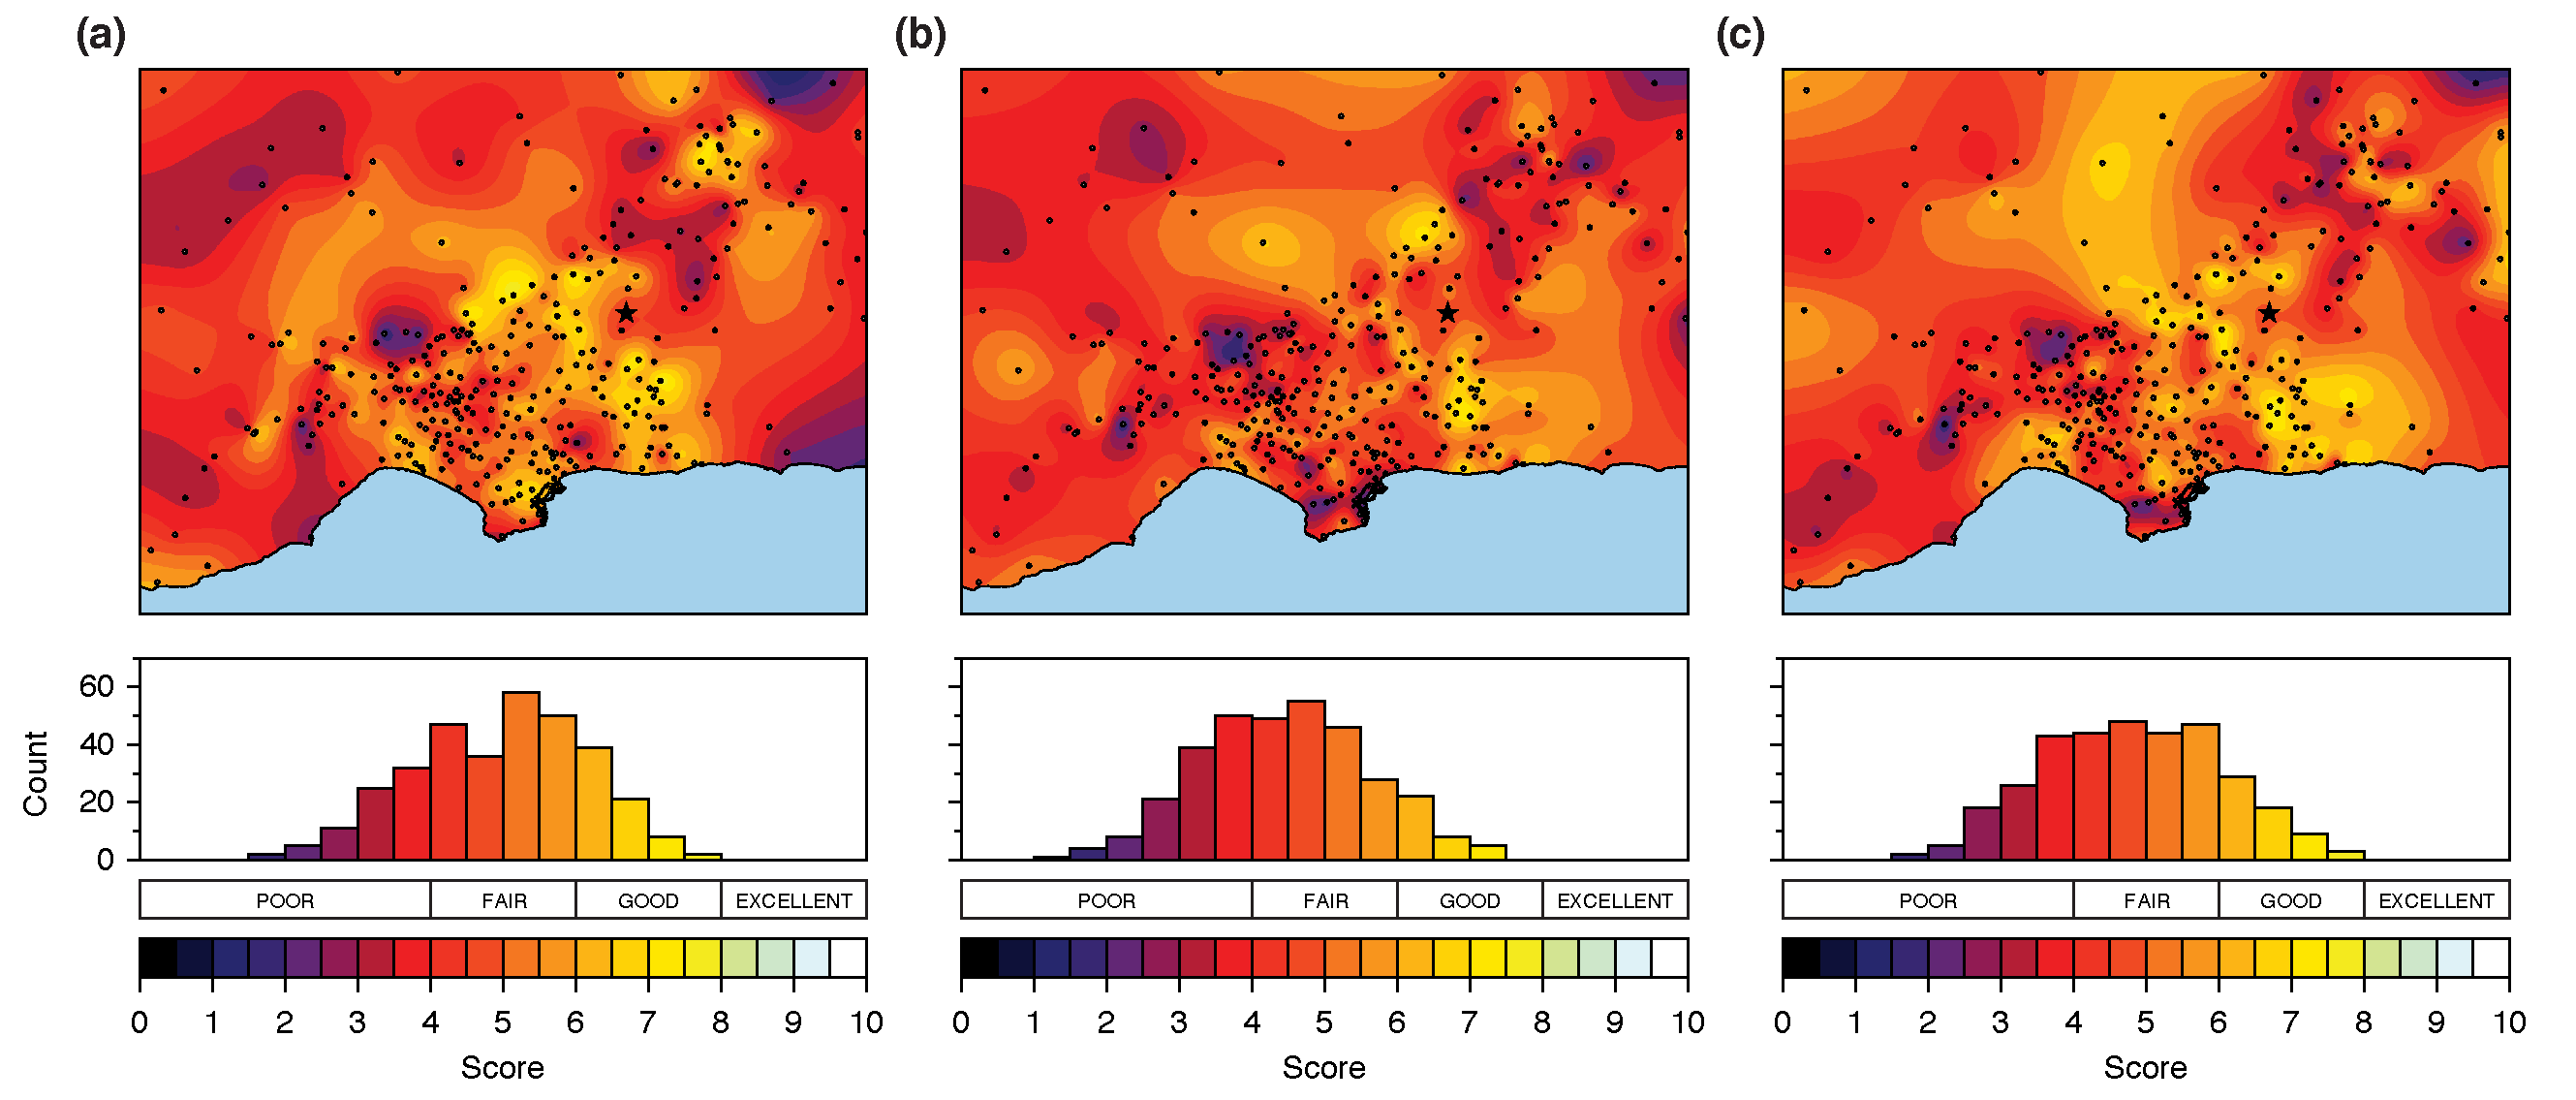
\includegraphics[width=\textwidth]{figures/pdf/figure-02}
    \caption{Validation results obtained by \citet{Taborda_2014_BSSA} in the form of GOF values across the region of interest obtained from comparisons between simulations for three different velocity models and data recorded at ground motion monitoring stations. The color version of this figure is available only in the electronic edition.}
    \label{fig:ref-gof-maps}
\end{figure*}
% 
\begin{figure}
    \centering
    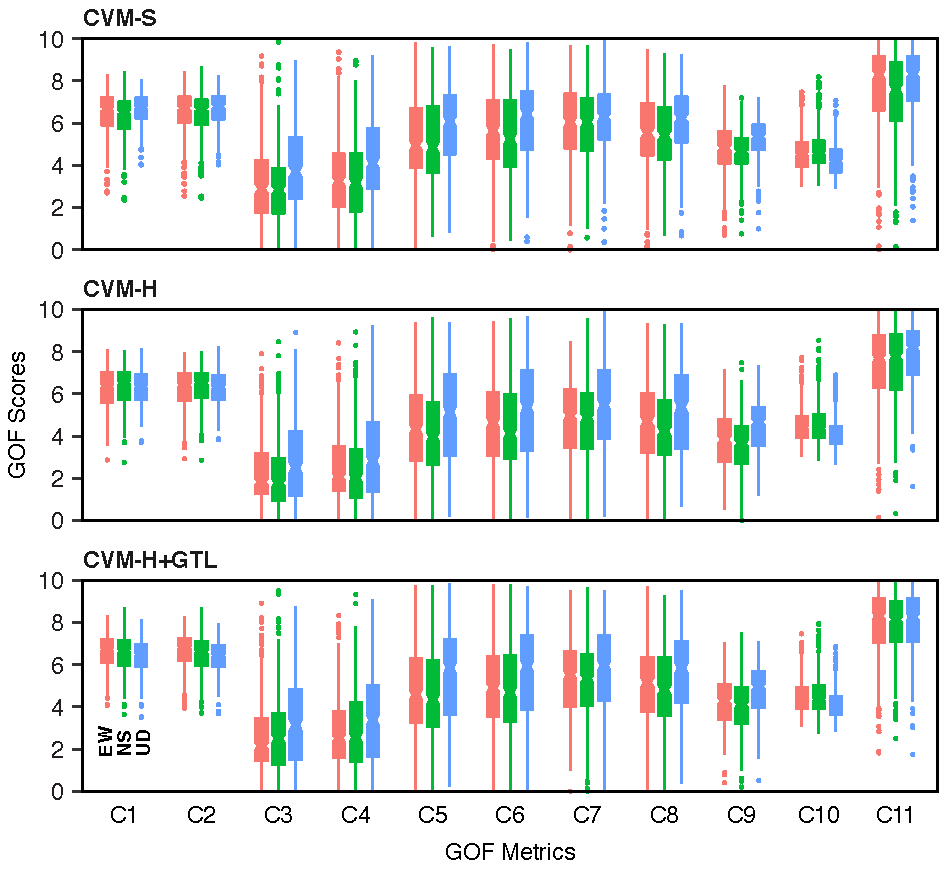
\includegraphics[width=\columnwidth]{figures/pdf/figure-03}
    \caption{Statistical distribution of the GOF dataset obtained from \citet{Taborda_2014_BSSA} shown in the form of box-plots for each metric (C1 through C11, see Table \ref{tab:metrics}), velocity model (CVM-S, CVM-H, and CVM-H+GTL), and component of motion (NS, EW, UD). In each case, the median is indicated by a notch in the box of the central quartiles, and the lines represent the interquartile range, with outliers shown as scattered dots. The color version of this figure is available only in the electronic edition.}
    \label{fig:data-box-plot}
\end{figure}

Here, we use the GOF scores obtained by \citet{Taborda_2014_BSSA} independently of the velocity models and/or the component of motions. Although at times we will make distinctions between the models and the components for visualization purposes, the clustering analysis to be described in the following section was done using the whole dataset of scores. The motivation behind this choice was that the dataset, as a sample of GOF values, was independent of the simulation and serves here as a generic set for the purpose of identifying the correlations that exist between the different metrics in Table \ref{tab:metrics}. As such, given the simulations for each velocity model (3), the motion components (3), and the number of stations used in the validation (336) gave us a large enough sample of 3,024 GOF scores. Figure \ref{fig:data-box-plot} illustrates this idea by comparing the statistical distribution of the broadband GOF scores of the simulations classified by velocity models and components. It is clear that although there are differences between them, these are negligible; in other words, the statistical distribution of results for each metric is about the same independently of model or component.

% ===========================================================================================
%
% OLD NAEEM VERSION
% 
% State of California is an earthquake prone region with a long history of seismicity. The Los Aneles basin, due to its unique geologic sediments, has been studied from different perspective. Numerous high resolution velocity models are developed mainly to conduct forward ground motion simulation. Occurrence of frequent moderate magnitude earthquakes made the Los Angeles basin as a natural laboratory for seismic  studies specially testing the forward ground motion simulation modeling. In a relatively recent study, \citet{Taborda_2014_BSSA} conducted a comprehensive study in order to assess the functionality of developed velocity models in the Los Angeles basin and surrounding areas. They simulated the 2008 Chino Hills earthquake using 3 velocity models including: CVM-S4, CVM-H, and CVM-H+GTL (for more details about these models see \citet{Taborda_2014_BSSA}.)
% They computed the GOF scores based on \citet{Anderson_2004_Proc}, with minor modification introduced by \citet{Taborda_2013_BSSA} as discussed in the validation section. Fig.~\ref{fig:epicenters} shows the location of the epicenter and seismic stations. 

% \begin{figure}
%     \centering
%     \includegraphics
%        % [width=\columnwidth]
%         [width=450px]
%         {figures/pdf/Figure_1}
%     \caption{(a) Region of interest and epicentral location of the 2008 $M_W ~ 5.4$ Chino Hills earthquake (highlighted). Focal mechanism is shown at the margin of the region of interest. Major quaternary faults in the area are shown in the back along with the main roads and county divisions. (b) Simulation area of interest. Dots indicate the location of the 336 stations considered in this study for validation. The main local and interstate roads are also shown here. In both panels, the background shows the hillshade topography of the region. The color version of this figure is available only in the electronic edition.}
%     \label{fig:epicenters}
% \end{figure}

% We use \citet{Taborda_2014_BSSA} database where they computed 11 scores for 3 different velocity models. In this study we only analyze the results for broadband which in this case is \feq{0.1}{4}. Fig.~\ref{fig:data_box_plot} shows the box plot of all data that we used in this study which we separate them in velocity models and components. In total we use $336 \times 3 \times 3 = 3024$ individual pair of data and synthetic.

% \begin{figure}
%     \centering
%     \includegraphics
%        % [width=\columnwidth]
%         [width=\textwidth]
%         {figures/pdf/Figure_2.pdf}
%     \caption{Box plot of data used in the study. Metrics are shown for C1 to C11 for 3 components and in separate plots for velocity models. Median of data are shown as a notch. Thick lines represent the IQR (Interquartile Range, Q3-Q1) of data. Outliers (data less than Q1-1.5*IQR and greater than Q3+1.5*IQR) are shown as scatter dots above and below plots if applicable.}
%     \label{fig:data_box_plot}
% \end{figure}

% As we explained before, we use all data set regardless of velocity models and components. However, distinguishing data for velocity model and components can answer the question that if the goodness of fit scores dependent on them. Addressing this research question is beyond the scope of this paper. We distinguish data based on velocity models and components only in presenting data or results.   

% Fig.~\ref{fig:data_density}  shows the density distribution of each score for CVM-S. The figure shows the variation of different metrics with components. Except in cross correlation (C10) in all metrics the up-down (UD) component scores are about the same or higher than horizontal components. 

% \begin{figure}
%     \centering
%     \includegraphics
%        % [width=\columnwidth]
%         [width=\textwidth]
%         {figures/pdf/Figure_3.pdf}
%     \caption{Distribution of data (only CVM-S) for different components in different scores based on different components. Each distribution has a unit area.}
%     \label{fig:data_density}
% \end{figure}









\section{Data Analysis Method} 
\label{sec:approach}

We are interested in developing a decision-making algorithm with a reduced and prioritized number of validation metrics based on previously acquired validation data (i.e., our dataset). A common method to do this is to identify rules with disjunctive characteristics in the form of a decision tree. The end-goal is to have a decision tree that leads to an outcome that is representative of the overall quality of the comparisons between two signals. In our case, we define such outcome in terms of four attributes representative of the quality of the validation, namely: poor, fair, good, and excellent.

In machine learning, decision trees are classified as a supervised learning method, and the first step towards designing them requires that the data be labeled according to their attributes. The inherent attribute of our data are the GOF value themselves, but because of the multiplicity of metrics and the lack of clarity about how these relate to each other, we need to add labels to the data that are in accordance with the outcome attributes, i.e., in terms of the predefined validation quality levels. We label the data in our dataset by means of a clustering process. 

There exist different methods for clustering data \citep[see Chapters 10 and 11 in][]{Han_2011_Book}, among which the \kmeans{} and constrained \kmeans{} clustering methods are the most widely used \citep{Jain_1999_ACMCS}. We note about these methods that the \kmeans{} approach is sensitive to the initial values chosen to be at the center of the clusters---especially in the case of data that are not clearly distinguishable---, whereas the constrained \kmeans{} method uses background knowledge to overcome this limitation. Because of its use of background information, the modified \kmeans{} method is considered as a semi-supervised process.

Once the data has been properly labeled, one can use a supervised approach to generate the decision tree through a recursive search for the best hypotheses to classify the outcome of the simulation based on a given sub-set of metrics. The following two sections explain the data processing analysis we have put in place to cluster our dataset and obtain the decision tree(s).


\subsection{Clustering}
\label{sec:clustering}

The first step towards obtaining a decision tree is to label the data according to their attributes. The inherent attribute of our data are the GOF values, but because of the multiplicity of metrics and lack of clarity about their relationships, we need to label the data according to the validation categories. We do this by means of a clustering process. 

Clustering is an unsupervised data-mining process used to group data in a multi-dimensional space based on their attributes \citep{Fayyad_1996_IEEE}. According to \citet{Jain_1999_ACMCS}, clustering can be classified in two categories: hierarchical and partitional. Technical details aside, the basic difference is that hierarchical algorithms create nested partitions, whereas partitional algorithms produce singular partitions. 

There is no single clustering process that can be applied to every dataset \citep{Dy_2004_MLR, Jain_1988_Book, Hartigan_1985_JOC}. Consequently, one needs to make choices. We use a partitional, distance-based method known as constrained \kmeans{}. The standard \kmeans{} method is a process for partitioning a $n$-dimensional population into $k$ clusters with a minimum within-cluster attributes variance \citep[e.g.,][]{Macqueen_1967_Proc}. Constrained \kmeans{} extends this method by allowing the use of background information in the form of clustering restrictions.

Given a $k$ number of clusters, where each cluster is identified by its center, the standard process starts by computing the distances of all other data-points to the center of the clusters, and grouping them based on their proximity to the clusters' centers. Once this is done, the center of each cluster is updated based on the average attributes of its data-points, and the process is repeated until the clusters become stable.

\begin{figure}[ht!]
	\centering
	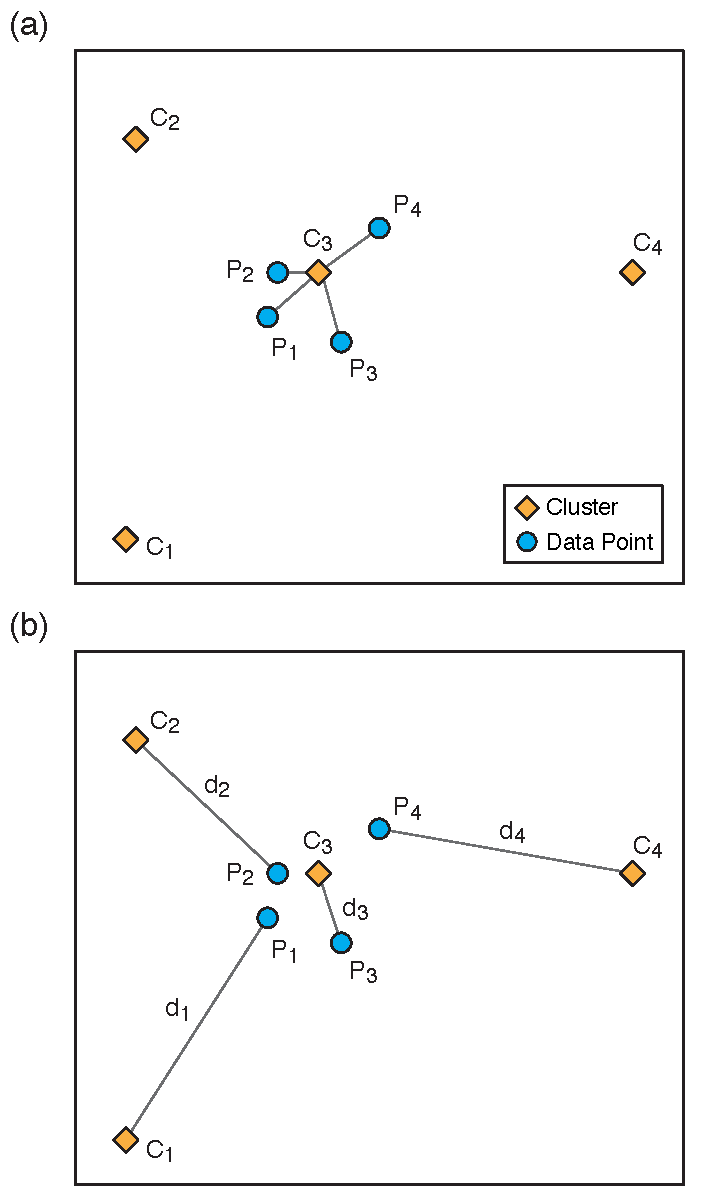
\includegraphics[width=\columnwidth]{figures/pdf/figure-04}
	\caption{Representation of the (a) ordinary, and (b) constrained \kmeans{} approaches for four data-points (P) and four cluster centers (C) in a 2D dataset space, where all the data-points are constrained to be cannot-link points. The color version of this figure is available only in the electronic edition.}
	\label{fig:k-means}
\end{figure}

This process is sensitive to the initial selection of the clusters and their centers. To mitigate this, constrained \kmeans{} introduces two types of constraints: must-link and cannot-link \citep{Wagstaff_2001_Proc}. The must-link constraint specifies instances in which two data-points must be linked, i.e., in the same cluster. The cannot-link constraint specifies instances in which data cannot be in the same cluster. This prevents the process from converging into a local minimum, and defines constrained \kmeans{} as a semi-supervised method. Figure \ref{fig:k-means} illustrates the differences between the standard and constrained \kmeans{} methods for a single clustering iteration on a small two-dimensional dataset.

In our implementation we limit the clustering to four validation categories: poor, fair, good, and excellent. The cluster centers are randomly selected at the start, but we apply constraints by adding 4 artificial stations with cannot-link conditions that are checked at the end of each iteration. These stations are associated with each type of cluster and have GOF scores equal to 3, 5, 7, and 9, across all metrics, thus they are representative of the validation categories. 

In the multi-dimensional space defined by the 11 GOF metrics used here, the distances are obtained using the Euclidean expression:
% 
\begin{equation}
	d(x_i, x_j) = \sqrt{ \sum_{l=1}^{n} \left( x_{i,l} - x_{j,l} \right)^2 } 
\end{equation}
% 
corresponding to the distance $d$ between the data-point $x_i$ and the cluster center $x_j$ in the $n$-dimensional domain, where $x_{i,l}$ is the $l$-th feature of the data-point $x_i$, and $x_{j,l}$ is the $l$-th feature of the cluster center $x_j$. It is, however, unpractical to expect the patterns defining the clusters to be observable across all features. Such high-dimensional issues are well known \citep[see, for instance,][]{Parsons_2004_ACM, Dy_2004_MLR}, and can be tackled using sub-spaces. Therefore, instead of analyzing all $2^{11}$ possible sub-spaces, we focus only on sub-spaces with 2, 3, and 4 dimensions, or features. In total, we analyze 550 sub-spaces, 55 sub-spaces with 2 features, 165 with 3, and 330 with 4.

Unfortunately, not all the sub-spaces will have clearly distinguishable clusters (i.e., some will not satisfy the cannot-link constraints even after a large number of iterations). Such sub-spaces are discarded, and all others are used to label the data. In an ideal case, each station will be labeled 550 times, and the final label is taken as the mode. For example, if after all the sub-spaces are accounted for, a station has labels $\left\{F, F, F, P, F, G, E, F, F\right\}$, where the labels $P$, $F$, $G$, and $E$ correspond to the poor, fair, good, and excellent category clusters, then such as station will be given a final label $F$. Once all the data is properly labeled, we proceed with the decision tree analysis.


% ===========================================================================================
%


% Although we do not expect to see the pattern that resulted from clustering using 11 features in presentation of only two, however, different studies show that the higher dimension reduce the effect of similarity based on distance. \citet{Parsons_2004_ACM} presented an illustrative example to show the effect of dimension in reducing the importance of the distance. Effect of higher dimensions in clustering has been well studied and many different methods are proposed to reduce this effect in the final results. Among them we can name  feature selection before, during, and after clustering, hybrid methods that use combination of methods to select the best subset of feature. \citet{Dy_2004_MLR} addressed two issues involved in developing an automated feature subset selection algorithm for unlabeled data. They illustrated the irrelevant and redundant features and proposed methods for evaluating candidate features using two performance criteria.

% Subspace analysis is another technique to address the challenges with higher dimensional data in clustering process. Subspace clustering is an extension of traditional clustering which looks for different pattern using subset of features.  \citet{Parsons_2004_ACM} provided a list of algorithm for conducting subspace clustering and also some potential applications for them. The most common factor among these algorithm is the process to find a group of best subspaces through optimization process. An n-dimensional dataset has $2^n$ subspaces where it could be very costly and time consuming to evaluate all of them.

% In this study we are interested in using those features who, in general, represent the simulation accuracy in 4 different categories. As a first step we use the constrained \kmeans{} clustering approach for all features, however, because of mentioned reasons the results are not easy to discuss or even evaluate. Although we have four groups of data, the question is which one should be considered as poor, fair, good, or excellent groups. Therefore, we apply a modified method of subspace clustering approach to cluster the stations. As we discussed earlier and presented in figures the constrained \kmeans{} method effectively put the stations in a cluster with considering the fact that our constrain stations should not be in the same cluster. High number of iteration leads the clustering process to follow the clustering concept that we are looking for which is clustering stations as poor, fair, good, and excellent. In our case number of possible subspace is $2^{11}$ where each features have two options wether belong to subspace or not. However, because of preserving the distance based criteria effects we limited the number of features in the subspace to be 2,3, and 4 features. Therefor we have 330,165, and 55 unique subspaces for 4D,3D, and 2D, respectively. We conduct a constrained \kmeans{} clustering analysis for each of these subspaces and repeat the algorithm. In some cases, it is not possible to distinguish all four cannot-link stations in different clusters. In this study we ignore these cases. We only use those combination of features that gives 4 unique clusters for the constraint points (hypothetical stations), therefore, we know for sure that all data within same cluster let's say with metric value 3, should be considered as poor. We also control the clusters to be consistent (we reformat numbers to assign cluster 1 to all group of stations that our first constraint belongs to them and so on). Finally, using 550 unique subspace clustering results, we assign the most frequent class to the station.





% and computes . These distances are then used as a criteria to determine the cluster to which cluster each data-point belongs. 

% ...


% \citet{Macqueen_1967_Proc} describes this method as a process for partitioning a $n$-dimensional population into $k$ sets on the basis of a sample. Its algorithm produces partitions that are reasonably efficient in the sense of within-class variance. It starts with a user defined number of clusters ($k$) and assigns a random mean value to each cluster (or randomly choose $k$ data-points and assigns them as cluster centers). After this, the algorithm computes the distances of all other data-points to the center of the cluster and uses the distance as a criteria to clustering the data points. Because the data resides in a multi-dimensional space (here defined by each metric), there are different ways of computing the distance of each data-point to the cluster's center. We use the Euclidean distance:
% % 
% \begin{equation}
% 	d(x_i, x_j) = \sqrt{ \sum_{k=1}^{n} \left( x_{i,k} - x_{j,k} \right)^2 } 
% 	\, ,
% \end{equation}
% % 
% where $n$ is the number of features and $d$ is the distance of $x_i$ and $x_j$ in $n$-$dimensional$ domain. 




% ===========================================================================================
%
% NEW TEXT PROVIDED BY NAEEM ON JAN 22
% Once the distance is computed, the algorithms labels the data based on the proximity of each point to each cluster, and computes the arithmetic mean value of the data for each cluster, and assigne that value as the updated location of each cluster's center. The algorithm repeats the steps unless the amount of updates among the cluster centers is less than a predefined tolerance value. The major problem with \kmeans{} algorithm is that it is sensitive to the selection of the initial partition and may converge to a local minimum of the criterion function value if the initial partition is not properly chosen. Another problem accompanying the use of \kmeans{} algorithm is the choice of the number of desired output clusters. \citep{Jain_1999_ACMCS}. Clustering is a subjective process. The same set of data items often needs to be partitioned differently for different application. In our application the number of clusters according to the literature is 4 (i.e., poor, fair, good, and excellent.) However, our initial attempts represents that the results are highly sensitive to the initial clusters' center. Therefore, we need to incorporate the experts knowlege in the process. 


% \citet{Wagstaff_2001_Proc}  demonstrated a modification of \kmeans{} clustering algorithm which uses the background information of the domain or dataset. The algorithm adds two types of constraints to the clustering including:
% 	% 
% 	\begin{itemize}
% 	\item{Must-link: constraints specify that two instances have to be in the same cluster.}
% 	\item{Cannot-link: constraints specify that two instance must not be placed in the same cluster.}
% 	\end{itemize} 
% 	% 
% The algorithm is described in detail in \citet{Wagstaff_2001_Proc}, however, in simple words, in the ordinary \kmeans{} process before assigning data to the closes cluster, it controls the must-link and cannot-link conditions. Therefore, in this case, the closest cluster's center is not necessarily the final cluster of the data.


% In a hypothetical assumption, if we have a pair of data and synthetic with GOF score of 3 for all metrics we could consider the overall simulation GOF as poor. This is also correct for 5,7, and 9 that we can assigne them fair, good, and excellent class, respectively. Therefore, we add 4 hypothetical stations into the dataset with GOF score of 3,5,7,and 9 for all metrics and we put them in cannot-link constraint. This assumption that originated from the experts knowledge, provides enough information to the algorithm to converge to the same final clusters and cluster centers after a reasonable amount of iteration. 

% Fig.~\ref{fig:con_kmeans} presents the difference between ordinary and constrained k-means clustering approach using 4 points and 4 cluster centers. Fig.~\ref{fig:con_kmeans}.a presents the \kmeans{} without constrained. According to the definition and the explanation in this section, the closest cluster center for each points will get the points. 	Fig.~\ref{fig:con_kmeans}.b represents the constrained \kmeans{} approach, where, the closest cluster center is not necessarily the final cluster. The data points can not be in the same cluster, in result,  we assign them to different clusters in this case to satisfy the Cannot-link criteria. The best configuration happens when we minimize the distance between cluster centers and points.

% ===========================================================================================
% 
% OLD STUFF DONE BY RICARDO FOR THE INTRO OF THIS SECTION
% 
% In machine learning, decision trees are classified as a supervised learning method, and the first step towards designing them requires that the data be labeled according to their attributes. The inherent attribute of our data are the GOF value themselves, but because of the multiplicity of metrics and the lack of clarity about how these relate to each other, we need to add labels to the data that are in accordance with the outcome attributes, i.e., in terms of the predefined validation quality levels. We label the data in our dataset by means of a clustering process. 

% There exist different methods for clustering data \citep[see Chapters 10 and 11 in][]{Han_2011_Book}, among which the \kmeans{} and constrained \kmeans{} clustering methods are the most widely used \citep{Jain_1999_ACMCS}. We note about these methods that the \kmeans{} approach is sensitive to the initial values chosen to be at the center of the clusters---especially in the case of data that are not clearly distinguishable---, whereas the constrained \kmeans{} method uses background knowledge to overcome this limitation. Because of its use of background information, the modified \kmeans{} method is considered as a semi-supervised process.





% ===========================================================================================
%
% SECOND ATTEMPT THAT WAS RECALLED BY NAEEM

% Once the distance is computed, the algorithms labels the data based on the proximity of each point to each cluster, computes the mean value of the data for each cluster, and updates the location of each cluster's center. \textcolor{red}{(How do we compute ``mean value'' and how do we recompute the ``center''? All what follows after this in the original text is too descriptive, and not specific enough. We need to go to the point and this is going in long description circles.)} 

% {\color{gray}
% 	The algorithm repeats the steps unless the amount of updates among the cluster centers is less than a tolerance value.  \kmeans{} clustering has been applied in different applications, however, there is no clustering technique that is universally applicable in uncovering the variety of structures present in multidimensional datasets. Therefore, clustering is a subjective process. The same set of data items often needs to be partitioned differently for different application. In result, it is essential for the user of a clustering algorithm to not only have a thorough understanding of the particular technique being utilized, but also to know the details of the data gathering process and to have some domain expertise; the more information the user has about the data at hand, the more likely the algorithm would be able to succeed in assessing its true class structure. Domain concept can play several roles in the clustering process, and a variety of choices are available to the practitioner \citep{Jain_1999_ACMCS}. 

% 	The major problem with \kmeans{} algorithm is that it is sensitive to the selection of the initial partition and may converge to a local minimum of the criterion function value if the initial partition is not properly chosen. Another problem accompanying the use of \kmeans{} algorithm is the choice of the number of desired output clusters. Several variant of the \kmeans{} algorithm have been reported in the literature. Some of them attempt to select a good initial partition so that the algorithm is more likely to find the global minimum value, another variation is to permit splitting and merging of the resulting clusters \citep{Jain_1999_ACMCS}. 

% 	In our application the number of clusters is not a problem and there is a consensus among researchers in the number of clusters (i.e., poor, fair, good, excellent), however, our initial attempts represent that the results are highly sensitive to the initial clusters' center. 

% 	Every clustering algorithm uses some type of knowledge either implicitly or explicitly. In this study the background knowledge is a series of hypothetical stations. We assume that there are four stations with score of 3, 5, 7, and 9 for all of their metrics. Based on the score limits in section.~\ref{validation_metrics} we know these stations belong to poor, fair, good, and excellent classes, respectively. These background knowledge could help the clustering processing to be in right direction regarding the fact that increasing dimension of data could increase noise in clustering and cause difficulty to better partitioning. \citet{Wagstaff_2001_Proc}  demonstrated a modification of \kmeans{} clustering algorithm which uses the background information of the domain or dataset. The algorithm adds two types of constraints to the clustering including:
% 	% 
% 	\begin{itemize}
% 	\item{Must-link: constraints specify that two instances have to be in the same cluster.}
% 	\item{Cannot-link: constraints specify that two instance must not be placed in the same cluster.}
% 	\end{itemize} 
% 	% 
% 	The algorithm is described in detail in \citet{Wagstaff_2001_Proc}, however, in simple words, in the ordinary \kmeans{} process before assigning data to the closes cluster, it controls the must-link and cannot-link conditions. Therefore, in this case, the closest cluster's center is not necessarily the final cluster of the data. Fig.~\ref{fig:con_kmeans} presents the difference between ordinary and constrained k-means clustering approach using 4 points and 4 cluster centers. Fig.~\ref{fig:con_kmeans}.a presents the \kmeans{} without constrained. According to the definition and the explanation in this section, the closest cluster center for each points will get the points.
	
% 	Fig.~\ref{fig:con_kmeans}.b represents the constrained \kmeans{} approach, where, the closest cluster center is not necessarily the final cluster. The data points can not be in the same cluster, in result,  we assign them to different clusters in this case to satisfy the Cannot-link criteria. The best configuration happens when we minimize the distance between cluster centers and points. Using this method at each step the algorithm redistribute the 4 hypothetical stations to satisfy the cannot-link constraint. The visual inspection of the figures also confirms the accuracy of the method. Doing this, in the next iteration this data manipulation leads the cluster center in a direction to have the hypothetical station in the cluster and loose those data that is in far other side direction of the hypothetical station. Therefore, the cluster tend to have all data that similar to the hypothetical station. \\
% 	The end product of the clustering process is groups of data. Analysis of these groups, individually, gives the idea about the clusters in terms of within class variation. In these analysis we mainly study the behavior of different features in each cluster and isolate only the most descriptive features to be used in the supervised classifier that assumes a given number of classes in the data set. In the next section we provide a basics of decision tree algorithm. 

% }

% In other words, the points cannot be in the same cluster. In the constrained \kmeans{} approach we redistribute the points such that the $\sum{d}$ becomes minimum.

% ===========================================================================================
%
% OLD NAEEM VERSION
% 
% Clustering is an unsupervised approach for grouping of data based on measure of similarity and it is considered as an exploratory activity as a part of data mining process \citep{Fayyad_1996_IEEE}. In each valid cluster, patterns are more similar in each other than they are to pattern belonging to a different cluster. Many clustering algorithms are developed for different application, however, study the difference of them is beyond the scope of this paper. In general, at the top level,  \citet{Jain_1999} distinguished the clustering approach into Hierarchical and Partitional approaches. Aside from differences in application and technical details in implementation, hierarchical methods produce nested series of partitions, while partitional methods produce only one. In this study we are interested in using partitional, distance based clustering algorithm, which is also known as \kmeans{} algorithm.  \citet{Macqueen_1967_Proc}  described a process for partitioning an $n$-$dimensional$ population into $k$ sets on the basis of a sample. The process appears to give partitions which are reasonably efficient in the sense of within-class variance. For numerical values, \kmeans{} algorithm starts with a user defined number of clusters (k) and assign a random mean value for each cluster (or randomly choose k data and assign them as cluster centers.) Then it computes the distance of data and cluster centers. A variety of distance measures are in use in different studies, however, we use the Euclidean distance through 

% \begin{equation}
% d(x_i,x_j)=\sqrt{\Sigma_{k=1}^{n}(x_{i,k} - x_{j,k})^2},
% \end{equation}

% where $n$ is the number of features and $d$ is the distance of $x_i$ and $x_j$ in $n$-$dimensional$ domain. After computing the distance of the points from each clusters' mean (center), the algorithm continues with labeling the data after the closest cluster. At the next iteration, it computes the mean value of data for each cluster and updates the clusters' centers. The algorithm repeats the steps unless the amount of updates among the cluster centers is less than a tolerance value.  \kmeans{} clustering has been applied in different applications, however, there is no clustering technique that is universally applicable in uncovering the variety of structures present in multidimensional datasets. Therefore, clustering is a subjective process. The same set of data items often needs to be partitioned differently for different application. In result, it is essential for the user of a clustering algorithm to not only have a thorough understanding of the particular technique being utilized, but also to know the details of the data gathering process and to have some domain expertise; the more information the user has about the data at hand, the more likely the algorithm would be able to succeed in assessing its true class structure. Domain concept can play several roles in the clustering process, and a variety of choices are available to the practitioner \citep{Jain_1999}. 

% The major problem with \kmeans{} algorithm is that it is sensitive to the selection of the initial partition and may converge to a local minimum of the criterion function value if the initial partition is not properly chosen. Another problem accompanying the use of \kmeans{} algorithm is the choice of the number of desired output clusters. Several variant of the \kmeans{} algorithm have been reported in the literature. Some of them attempt to select a good initial partition so that the algorithm is more likely to find the global minimum value, another variation is to permit splitting and merging of the resulting clusters \citep{Jain_1999}. 

% In our application the number of clusters is not a problem and there is a consensus among researchers in the number of clusters (i.e., poor, fair, good, excellent), however, our initial attempts represent that the results are highly sensitive to the initial clusters' center. 

% Every clustering algorithm uses some type of knowledge either implicitly or explicitly. In this study the background knowledge is a series of hypothetical stations. We assume that there are four stations with score of 3, 5, 7, and 9 for all of their metrics. Based on the score limits in section.~\ref{validation_metrics} we know these stations belong to poor, fair, good, and excellent classes, respectively. These background knowledge could help the clustering processing to be in right direction regarding the fact that increasing dimension of data could increase noise in clustering and cause difficulty to better partitioning. \citet{Wagstaff_2001_Proc}  demonstrated a modification of \kmeans{} clustering algorithm which uses the background information of the domain or dataset. The algorithm adds two types of constraints to the clustering including:\\
% \begin{itemize}
% \item{Must-link: constraints specify that two instances have to be in the same cluster.}
% \item{Cannot-link: constraints specify that two instance must not be placed in the same cluster.}
% \end{itemize} 
% The algorithm is described in detail in \citet{Wagstaff_2001_Proc}, however, in simple words, in the ordinary \kmeans{} process before assigning data to the closes cluster, it controls the must-link and cannot-link conditions. Therefore, in this case, the closest cluster's center is not necessarily the final cluster of the data. Fig.~\ref{fig:con_kmeans} presents the difference between ordinary and constrained k-means clustering approach using 4 points and 4 cluster centers. Fig.~\ref{fig:con_kmeans}.a presents the \kmeans{} without constrained. According to the definition and the explanation in this section, the closest cluster center for each points will get the points.
% Fig.~\ref{fig:con_kmeans}.b represents the constrained \kmeans{} approach, where, the closest cluster center is not necessarily the final cluster. The data points can not be in the same cluster, in result,  we assign them to different clusters in this case to satisfy the Cannot-link criteria. The best configuration happens when we minimize the distance between cluster centers and points. Using this method at each step the algorithm redistribute the 4 hypothetical stations to satisfy the cannot-link constraint. The visual inspection of the figures also confirms the accuracy of the method. Doing this, in the next iteration this data manipulation leads the cluster center in a direction to have the hypothetical station in the cluster and loose those data that is in far other side direction of the hypothetical station. Therefore, the cluster tend to have all data that similar to the hypothetical station. \\
% The end product of the clustering process is groups of data. Analysis of these groups, individually, gives the idea about the clusters in terms of within class variation. In these analysis we mainly study the behavior of different features in each cluster and isolate only the most descriptive features to be used in the supervised classifier that assumes a given number of classes in the data set. In the next section we provide a basics of decision tree algorithm. 


% \begin{figure}
%     \centering
%     \includegraphics
%       %  [width=\columnwidth]
%         [width=200px]
%         {figures/pdf/Figure_4.pdf}
%     \caption{ Representation of ordinary (a) and constrained (b) \kmeans{} approach. There are four data points (p) and four cluster centers (c) as a sample of $2$-$Dimensional$ dataset. All points are defined as cannot-link constraints. In other words, the points cannot be in the same cluster. In the constrained \kmeans{} approach we redistribute the points such that the $\sum{d}$ becomes minimum.}
%     \label{fig:con_kmeans}
% \end{figure}





% =========================================================================================================================
% 
% NAEEM NEW SUGGESTION
% 
% Prioritized, reduced number of validation metrics requires developing a decision-making algorithm. A common method to do this is to identify rules with disjunctive characteristics in the form of a decision tree. Decision tree is considered as a supervised learning method. Therefore, we need to know the overall GOF of each observation in the dataset. Or in other words if we consider the simulation process for that specific station and component as poor, fair, good, or excellent process.  Therefore, the first step in such an approach requires that the data be labeled according to their attributes. The inherent attribute of our data is the GOF value, but need to label the data in terms of the outcome attribute. Generating labels for data is mainly possible through a clustering process. There exist different methods for clustering data (see Chapter 10 and 11 of Han 2011). The k-means and constrained k -means clustering methods are among the most widely used Ease of implementation, simplicity, efficiency, and empirical success are the main reasons for its popularity (Jain 2010). We note about these methods that the k –means approach is sensitive to the initial values chosen as the center of the clusters—especially in the case of data that are not clearly distinguishable—, whereas the constrained k –means method uses background knowledge to overcome this limitation. Because of its used of background information, the modified k -means method is considered as a semi-supervised process. Once the data has been properly labeled, one can use a supervised approach to generate the decision tree that can serve as a prediction model for the outcome. In essence, the process of designing the decision tree is a search for the best hypothesis to classify the outcome of the simulation, i.e., the similarity between synthetic and recorded seismograms, based on a given sub-set of metrics. The following two sections explain the data processing analysis we have put in place to achieve this.

% =========================================================================================================================
% 
% RICARDO FIRST PASS

% In order to study the relationships that exist between the different validation metrics and offer a prioritized, reduced number of metrics that can help predict validation results, we need to identify and classify patterns in the dataset. A common method to do this is to identify rules with disjunctive characteristics in the form of a decision tree. Among the available approaches used to design such a tree there are machine learning methods that use supervised and unsupervised learning. The first step in such an approach requires that the data be labeled according to their attributes. The inherent attribute of our data is the GOF value, but need to label the data in terms of the outcome attribute. Following common practice, in our case, we want to label the dataset values as poor, fair, good, or excellent.

% Generating labels for data in an automated way is possible through a clustering process. There exist different methods for clustering data (see \textcolor{red}{a reference about clustering}). The \kmeans{} and modified \kmeans{} clustering methods are among the most widely used (\textcolor{red}{a reference to back up this statement}). We note about these methods that the \kmeans{} approach is sensitive to the initial values chosen at the center of the clusters---especially in the case of data that are not clearly distinguishable---, whereas the modified \kmeans{} method uses background knowledge to overcome this limitation. Because of its used of background information, the modified \kmeans{} method is considered as a semi-supervised process.

% Once the data has been properly labeled, one can use a supervised approach to generate the decision tree that can serve as a prediction model for the outcome. In essence, the process of designing the decision tree is a search for the best hypothesis to classify the outcome of the simulation, i.e., the similarity between synthetic and recorded seismograms, based on a given sub-set of metrics. The following two sections explain the data processing analysis we have put in place to achieve this.

% 
\subsection{Clustering}
\label{sec:clustering}

The first step towards obtaining a decision tree is to label the data according to their attributes. The inherent attribute of our data are the GOF values, but because of the multiplicity of metrics and lack of clarity about their relationships, we need to label the data according to the validation categories. We do this by means of a clustering process. 

Clustering is an unsupervised data-mining process used to group data in a multi-dimensional space based on their attributes \citep{Fayyad_1996_IEEE}. According to \citet{Jain_1999_ACMCS}, clustering can be classified in two categories: hierarchical and partitional. Technical details aside, the basic difference is that hierarchical algorithms create nested partitions, whereas partitional algorithms produce singular partitions. 

There is no single clustering process that can be applied to every dataset \citep{Dy_2004_MLR, Jain_1988_Book, Hartigan_1985_JOC}. Consequently, one needs to make choices. We use a partitional, distance-based method known as constrained \kmeans{}. The standard \kmeans{} method is a process for partitioning a $n$-dimensional population into $k$ clusters with a minimum within-cluster attributes variance \citep[e.g.,][]{Macqueen_1967_Proc}. Constrained \kmeans{} extends this method by allowing the use of background information in the form of clustering restrictions.

Given a $k$ number of clusters, where each cluster is identified by its center, the standard process starts by computing the distances of all other data-points to the center of the clusters, and grouping them based on their proximity to the clusters' centers. Once this is done, the center of each cluster is updated based on the average attributes of its data-points, and the process is repeated until the clusters become stable.

\begin{figure}[ht!]
	\centering
	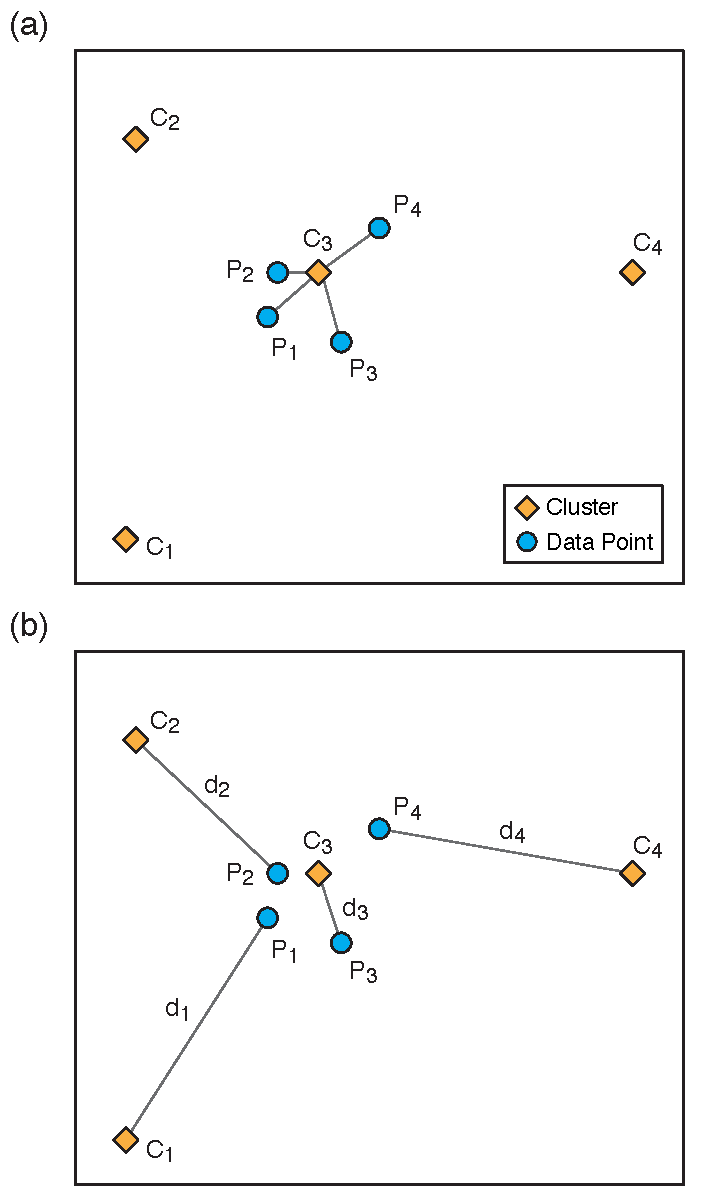
\includegraphics[width=\columnwidth]{figures/pdf/figure-04}
	\caption{Representation of the (a) ordinary, and (b) constrained \kmeans{} approaches for four data-points (P) and four cluster centers (C) in a 2D dataset space, where all the data-points are constrained to be cannot-link points. The color version of this figure is available only in the electronic edition.}
	\label{fig:k-means}
\end{figure}

This process is sensitive to the initial selection of the clusters and their centers. To mitigate this, constrained \kmeans{} introduces two types of constraints: must-link and cannot-link \citep{Wagstaff_2001_Proc}. The must-link constraint specifies instances in which two data-points must be linked, i.e., in the same cluster. The cannot-link constraint specifies instances in which data cannot be in the same cluster. This prevents the process from converging into a local minimum, and defines constrained \kmeans{} as a semi-supervised method. Figure \ref{fig:k-means} illustrates the differences between the standard and constrained \kmeans{} methods for a single clustering iteration on a small two-dimensional dataset.

In our implementation we limit the clustering to four validation categories: poor, fair, good, and excellent. The cluster centers are randomly selected at the start, but we apply constraints by adding 4 artificial stations with cannot-link conditions that are checked at the end of each iteration. These stations are associated with each type of cluster and have GOF scores equal to 3, 5, 7, and 9, across all metrics, thus they are representative of the validation categories. 

In the multi-dimensional space defined by the 11 GOF metrics used here, the distances are obtained using the Euclidean expression:
% 
\begin{equation}
	d(x_i, x_j) = \sqrt{ \sum_{l=1}^{n} \left( x_{i,l} - x_{j,l} \right)^2 } 
\end{equation}
% 
corresponding to the distance $d$ between the data-point $x_i$ and the cluster center $x_j$ in the $n$-dimensional domain, where $x_{i,l}$ is the $l$-th feature of the data-point $x_i$, and $x_{j,l}$ is the $l$-th feature of the cluster center $x_j$. It is, however, unpractical to expect the patterns defining the clusters to be observable across all features. Such high-dimensional issues are well known \citep[see, for instance,][]{Parsons_2004_ACM, Dy_2004_MLR}, and can be tackled using sub-spaces. Therefore, instead of analyzing all $2^{11}$ possible sub-spaces, we focus only on sub-spaces with 2, 3, and 4 dimensions, or features. In total, we analyze 550 sub-spaces, 55 sub-spaces with 2 features, 165 with 3, and 330 with 4.

Unfortunately, not all the sub-spaces will have clearly distinguishable clusters (i.e., some will not satisfy the cannot-link constraints even after a large number of iterations). Such sub-spaces are discarded, and all others are used to label the data. In an ideal case, each station will be labeled 550 times, and the final label is taken as the mode. For example, if after all the sub-spaces are accounted for, a station has labels $\left\{F, F, F, P, F, G, E, F, F\right\}$, where the labels $P$, $F$, $G$, and $E$ correspond to the poor, fair, good, and excellent category clusters, then such as station will be given a final label $F$. Once all the data is properly labeled, we proceed with the decision tree analysis.


% ===========================================================================================
%


% Although we do not expect to see the pattern that resulted from clustering using 11 features in presentation of only two, however, different studies show that the higher dimension reduce the effect of similarity based on distance. \citet{Parsons_2004_ACM} presented an illustrative example to show the effect of dimension in reducing the importance of the distance. Effect of higher dimensions in clustering has been well studied and many different methods are proposed to reduce this effect in the final results. Among them we can name  feature selection before, during, and after clustering, hybrid methods that use combination of methods to select the best subset of feature. \citet{Dy_2004_MLR} addressed two issues involved in developing an automated feature subset selection algorithm for unlabeled data. They illustrated the irrelevant and redundant features and proposed methods for evaluating candidate features using two performance criteria.

% Subspace analysis is another technique to address the challenges with higher dimensional data in clustering process. Subspace clustering is an extension of traditional clustering which looks for different pattern using subset of features.  \citet{Parsons_2004_ACM} provided a list of algorithm for conducting subspace clustering and also some potential applications for them. The most common factor among these algorithm is the process to find a group of best subspaces through optimization process. An n-dimensional dataset has $2^n$ subspaces where it could be very costly and time consuming to evaluate all of them.

% In this study we are interested in using those features who, in general, represent the simulation accuracy in 4 different categories. As a first step we use the constrained \kmeans{} clustering approach for all features, however, because of mentioned reasons the results are not easy to discuss or even evaluate. Although we have four groups of data, the question is which one should be considered as poor, fair, good, or excellent groups. Therefore, we apply a modified method of subspace clustering approach to cluster the stations. As we discussed earlier and presented in figures the constrained \kmeans{} method effectively put the stations in a cluster with considering the fact that our constrain stations should not be in the same cluster. High number of iteration leads the clustering process to follow the clustering concept that we are looking for which is clustering stations as poor, fair, good, and excellent. In our case number of possible subspace is $2^{11}$ where each features have two options wether belong to subspace or not. However, because of preserving the distance based criteria effects we limited the number of features in the subspace to be 2,3, and 4 features. Therefor we have 330,165, and 55 unique subspaces for 4D,3D, and 2D, respectively. We conduct a constrained \kmeans{} clustering analysis for each of these subspaces and repeat the algorithm. In some cases, it is not possible to distinguish all four cannot-link stations in different clusters. In this study we ignore these cases. We only use those combination of features that gives 4 unique clusters for the constraint points (hypothetical stations), therefore, we know for sure that all data within same cluster let's say with metric value 3, should be considered as poor. We also control the clusters to be consistent (we reformat numbers to assign cluster 1 to all group of stations that our first constraint belongs to them and so on). Finally, using 550 unique subspace clustering results, we assign the most frequent class to the station.





% and computes . These distances are then used as a criteria to determine the cluster to which cluster each data-point belongs. 

% ...


% \citet{Macqueen_1967_Proc} describes this method as a process for partitioning a $n$-dimensional population into $k$ sets on the basis of a sample. Its algorithm produces partitions that are reasonably efficient in the sense of within-class variance. It starts with a user defined number of clusters ($k$) and assigns a random mean value to each cluster (or randomly choose $k$ data-points and assigns them as cluster centers). After this, the algorithm computes the distances of all other data-points to the center of the cluster and uses the distance as a criteria to clustering the data points. Because the data resides in a multi-dimensional space (here defined by each metric), there are different ways of computing the distance of each data-point to the cluster's center. We use the Euclidean distance:
% % 
% \begin{equation}
% 	d(x_i, x_j) = \sqrt{ \sum_{k=1}^{n} \left( x_{i,k} - x_{j,k} \right)^2 } 
% 	\, ,
% \end{equation}
% % 
% where $n$ is the number of features and $d$ is the distance of $x_i$ and $x_j$ in $n$-$dimensional$ domain. 




% ===========================================================================================
%
% NEW TEXT PROVIDED BY NAEEM ON JAN 22
% Once the distance is computed, the algorithms labels the data based on the proximity of each point to each cluster, and computes the arithmetic mean value of the data for each cluster, and assigne that value as the updated location of each cluster's center. The algorithm repeats the steps unless the amount of updates among the cluster centers is less than a predefined tolerance value. The major problem with \kmeans{} algorithm is that it is sensitive to the selection of the initial partition and may converge to a local minimum of the criterion function value if the initial partition is not properly chosen. Another problem accompanying the use of \kmeans{} algorithm is the choice of the number of desired output clusters. \citep{Jain_1999_ACMCS}. Clustering is a subjective process. The same set of data items often needs to be partitioned differently for different application. In our application the number of clusters according to the literature is 4 (i.e., poor, fair, good, and excellent.) However, our initial attempts represents that the results are highly sensitive to the initial clusters' center. Therefore, we need to incorporate the experts knowlege in the process. 


% \citet{Wagstaff_2001_Proc}  demonstrated a modification of \kmeans{} clustering algorithm which uses the background information of the domain or dataset. The algorithm adds two types of constraints to the clustering including:
% 	% 
% 	\begin{itemize}
% 	\item{Must-link: constraints specify that two instances have to be in the same cluster.}
% 	\item{Cannot-link: constraints specify that two instance must not be placed in the same cluster.}
% 	\end{itemize} 
% 	% 
% The algorithm is described in detail in \citet{Wagstaff_2001_Proc}, however, in simple words, in the ordinary \kmeans{} process before assigning data to the closes cluster, it controls the must-link and cannot-link conditions. Therefore, in this case, the closest cluster's center is not necessarily the final cluster of the data.


% In a hypothetical assumption, if we have a pair of data and synthetic with GOF score of 3 for all metrics we could consider the overall simulation GOF as poor. This is also correct for 5,7, and 9 that we can assigne them fair, good, and excellent class, respectively. Therefore, we add 4 hypothetical stations into the dataset with GOF score of 3,5,7,and 9 for all metrics and we put them in cannot-link constraint. This assumption that originated from the experts knowledge, provides enough information to the algorithm to converge to the same final clusters and cluster centers after a reasonable amount of iteration. 

% Fig.~\ref{fig:con_kmeans} presents the difference between ordinary and constrained k-means clustering approach using 4 points and 4 cluster centers. Fig.~\ref{fig:con_kmeans}.a presents the \kmeans{} without constrained. According to the definition and the explanation in this section, the closest cluster center for each points will get the points. 	Fig.~\ref{fig:con_kmeans}.b represents the constrained \kmeans{} approach, where, the closest cluster center is not necessarily the final cluster. The data points can not be in the same cluster, in result,  we assign them to different clusters in this case to satisfy the Cannot-link criteria. The best configuration happens when we minimize the distance between cluster centers and points.

% ===========================================================================================
% 
% OLD STUFF DONE BY RICARDO FOR THE INTRO OF THIS SECTION
% 
% In machine learning, decision trees are classified as a supervised learning method, and the first step towards designing them requires that the data be labeled according to their attributes. The inherent attribute of our data are the GOF value themselves, but because of the multiplicity of metrics and the lack of clarity about how these relate to each other, we need to add labels to the data that are in accordance with the outcome attributes, i.e., in terms of the predefined validation quality levels. We label the data in our dataset by means of a clustering process. 

% There exist different methods for clustering data \citep[see Chapters 10 and 11 in][]{Han_2011_Book}, among which the \kmeans{} and constrained \kmeans{} clustering methods are the most widely used \citep{Jain_1999_ACMCS}. We note about these methods that the \kmeans{} approach is sensitive to the initial values chosen to be at the center of the clusters---especially in the case of data that are not clearly distinguishable---, whereas the constrained \kmeans{} method uses background knowledge to overcome this limitation. Because of its use of background information, the modified \kmeans{} method is considered as a semi-supervised process.





% ===========================================================================================
%
% SECOND ATTEMPT THAT WAS RECALLED BY NAEEM

% Once the distance is computed, the algorithms labels the data based on the proximity of each point to each cluster, computes the mean value of the data for each cluster, and updates the location of each cluster's center. \textcolor{red}{(How do we compute ``mean value'' and how do we recompute the ``center''? All what follows after this in the original text is too descriptive, and not specific enough. We need to go to the point and this is going in long description circles.)} 

% {\color{gray}
% 	The algorithm repeats the steps unless the amount of updates among the cluster centers is less than a tolerance value.  \kmeans{} clustering has been applied in different applications, however, there is no clustering technique that is universally applicable in uncovering the variety of structures present in multidimensional datasets. Therefore, clustering is a subjective process. The same set of data items often needs to be partitioned differently for different application. In result, it is essential for the user of a clustering algorithm to not only have a thorough understanding of the particular technique being utilized, but also to know the details of the data gathering process and to have some domain expertise; the more information the user has about the data at hand, the more likely the algorithm would be able to succeed in assessing its true class structure. Domain concept can play several roles in the clustering process, and a variety of choices are available to the practitioner \citep{Jain_1999_ACMCS}. 

% 	The major problem with \kmeans{} algorithm is that it is sensitive to the selection of the initial partition and may converge to a local minimum of the criterion function value if the initial partition is not properly chosen. Another problem accompanying the use of \kmeans{} algorithm is the choice of the number of desired output clusters. Several variant of the \kmeans{} algorithm have been reported in the literature. Some of them attempt to select a good initial partition so that the algorithm is more likely to find the global minimum value, another variation is to permit splitting and merging of the resulting clusters \citep{Jain_1999_ACMCS}. 

% 	In our application the number of clusters is not a problem and there is a consensus among researchers in the number of clusters (i.e., poor, fair, good, excellent), however, our initial attempts represent that the results are highly sensitive to the initial clusters' center. 

% 	Every clustering algorithm uses some type of knowledge either implicitly or explicitly. In this study the background knowledge is a series of hypothetical stations. We assume that there are four stations with score of 3, 5, 7, and 9 for all of their metrics. Based on the score limits in section.~\ref{validation_metrics} we know these stations belong to poor, fair, good, and excellent classes, respectively. These background knowledge could help the clustering processing to be in right direction regarding the fact that increasing dimension of data could increase noise in clustering and cause difficulty to better partitioning. \citet{Wagstaff_2001_Proc}  demonstrated a modification of \kmeans{} clustering algorithm which uses the background information of the domain or dataset. The algorithm adds two types of constraints to the clustering including:
% 	% 
% 	\begin{itemize}
% 	\item{Must-link: constraints specify that two instances have to be in the same cluster.}
% 	\item{Cannot-link: constraints specify that two instance must not be placed in the same cluster.}
% 	\end{itemize} 
% 	% 
% 	The algorithm is described in detail in \citet{Wagstaff_2001_Proc}, however, in simple words, in the ordinary \kmeans{} process before assigning data to the closes cluster, it controls the must-link and cannot-link conditions. Therefore, in this case, the closest cluster's center is not necessarily the final cluster of the data. Fig.~\ref{fig:con_kmeans} presents the difference between ordinary and constrained k-means clustering approach using 4 points and 4 cluster centers. Fig.~\ref{fig:con_kmeans}.a presents the \kmeans{} without constrained. According to the definition and the explanation in this section, the closest cluster center for each points will get the points.
	
% 	Fig.~\ref{fig:con_kmeans}.b represents the constrained \kmeans{} approach, where, the closest cluster center is not necessarily the final cluster. The data points can not be in the same cluster, in result,  we assign them to different clusters in this case to satisfy the Cannot-link criteria. The best configuration happens when we minimize the distance between cluster centers and points. Using this method at each step the algorithm redistribute the 4 hypothetical stations to satisfy the cannot-link constraint. The visual inspection of the figures also confirms the accuracy of the method. Doing this, in the next iteration this data manipulation leads the cluster center in a direction to have the hypothetical station in the cluster and loose those data that is in far other side direction of the hypothetical station. Therefore, the cluster tend to have all data that similar to the hypothetical station. \\
% 	The end product of the clustering process is groups of data. Analysis of these groups, individually, gives the idea about the clusters in terms of within class variation. In these analysis we mainly study the behavior of different features in each cluster and isolate only the most descriptive features to be used in the supervised classifier that assumes a given number of classes in the data set. In the next section we provide a basics of decision tree algorithm. 

% }

% In other words, the points cannot be in the same cluster. In the constrained \kmeans{} approach we redistribute the points such that the $\sum{d}$ becomes minimum.

% ===========================================================================================
%
% OLD NAEEM VERSION
% 
% Clustering is an unsupervised approach for grouping of data based on measure of similarity and it is considered as an exploratory activity as a part of data mining process \citep{Fayyad_1996_IEEE}. In each valid cluster, patterns are more similar in each other than they are to pattern belonging to a different cluster. Many clustering algorithms are developed for different application, however, study the difference of them is beyond the scope of this paper. In general, at the top level,  \citet{Jain_1999} distinguished the clustering approach into Hierarchical and Partitional approaches. Aside from differences in application and technical details in implementation, hierarchical methods produce nested series of partitions, while partitional methods produce only one. In this study we are interested in using partitional, distance based clustering algorithm, which is also known as \kmeans{} algorithm.  \citet{Macqueen_1967_Proc}  described a process for partitioning an $n$-$dimensional$ population into $k$ sets on the basis of a sample. The process appears to give partitions which are reasonably efficient in the sense of within-class variance. For numerical values, \kmeans{} algorithm starts with a user defined number of clusters (k) and assign a random mean value for each cluster (or randomly choose k data and assign them as cluster centers.) Then it computes the distance of data and cluster centers. A variety of distance measures are in use in different studies, however, we use the Euclidean distance through 

% \begin{equation}
% d(x_i,x_j)=\sqrt{\Sigma_{k=1}^{n}(x_{i,k} - x_{j,k})^2},
% \end{equation}

% where $n$ is the number of features and $d$ is the distance of $x_i$ and $x_j$ in $n$-$dimensional$ domain. After computing the distance of the points from each clusters' mean (center), the algorithm continues with labeling the data after the closest cluster. At the next iteration, it computes the mean value of data for each cluster and updates the clusters' centers. The algorithm repeats the steps unless the amount of updates among the cluster centers is less than a tolerance value.  \kmeans{} clustering has been applied in different applications, however, there is no clustering technique that is universally applicable in uncovering the variety of structures present in multidimensional datasets. Therefore, clustering is a subjective process. The same set of data items often needs to be partitioned differently for different application. In result, it is essential for the user of a clustering algorithm to not only have a thorough understanding of the particular technique being utilized, but also to know the details of the data gathering process and to have some domain expertise; the more information the user has about the data at hand, the more likely the algorithm would be able to succeed in assessing its true class structure. Domain concept can play several roles in the clustering process, and a variety of choices are available to the practitioner \citep{Jain_1999}. 

% The major problem with \kmeans{} algorithm is that it is sensitive to the selection of the initial partition and may converge to a local minimum of the criterion function value if the initial partition is not properly chosen. Another problem accompanying the use of \kmeans{} algorithm is the choice of the number of desired output clusters. Several variant of the \kmeans{} algorithm have been reported in the literature. Some of them attempt to select a good initial partition so that the algorithm is more likely to find the global minimum value, another variation is to permit splitting and merging of the resulting clusters \citep{Jain_1999}. 

% In our application the number of clusters is not a problem and there is a consensus among researchers in the number of clusters (i.e., poor, fair, good, excellent), however, our initial attempts represent that the results are highly sensitive to the initial clusters' center. 

% Every clustering algorithm uses some type of knowledge either implicitly or explicitly. In this study the background knowledge is a series of hypothetical stations. We assume that there are four stations with score of 3, 5, 7, and 9 for all of their metrics. Based on the score limits in section.~\ref{validation_metrics} we know these stations belong to poor, fair, good, and excellent classes, respectively. These background knowledge could help the clustering processing to be in right direction regarding the fact that increasing dimension of data could increase noise in clustering and cause difficulty to better partitioning. \citet{Wagstaff_2001_Proc}  demonstrated a modification of \kmeans{} clustering algorithm which uses the background information of the domain or dataset. The algorithm adds two types of constraints to the clustering including:\\
% \begin{itemize}
% \item{Must-link: constraints specify that two instances have to be in the same cluster.}
% \item{Cannot-link: constraints specify that two instance must not be placed in the same cluster.}
% \end{itemize} 
% The algorithm is described in detail in \citet{Wagstaff_2001_Proc}, however, in simple words, in the ordinary \kmeans{} process before assigning data to the closes cluster, it controls the must-link and cannot-link conditions. Therefore, in this case, the closest cluster's center is not necessarily the final cluster of the data. Fig.~\ref{fig:con_kmeans} presents the difference between ordinary and constrained k-means clustering approach using 4 points and 4 cluster centers. Fig.~\ref{fig:con_kmeans}.a presents the \kmeans{} without constrained. According to the definition and the explanation in this section, the closest cluster center for each points will get the points.
% Fig.~\ref{fig:con_kmeans}.b represents the constrained \kmeans{} approach, where, the closest cluster center is not necessarily the final cluster. The data points can not be in the same cluster, in result,  we assign them to different clusters in this case to satisfy the Cannot-link criteria. The best configuration happens when we minimize the distance between cluster centers and points. Using this method at each step the algorithm redistribute the 4 hypothetical stations to satisfy the cannot-link constraint. The visual inspection of the figures also confirms the accuracy of the method. Doing this, in the next iteration this data manipulation leads the cluster center in a direction to have the hypothetical station in the cluster and loose those data that is in far other side direction of the hypothetical station. Therefore, the cluster tend to have all data that similar to the hypothetical station. \\
% The end product of the clustering process is groups of data. Analysis of these groups, individually, gives the idea about the clusters in terms of within class variation. In these analysis we mainly study the behavior of different features in each cluster and isolate only the most descriptive features to be used in the supervised classifier that assumes a given number of classes in the data set. In the next section we provide a basics of decision tree algorithm. 


% \begin{figure}
%     \centering
%     \includegraphics
%       %  [width=\columnwidth]
%         [width=200px]
%         {figures/pdf/Figure_4.pdf}
%     \caption{ Representation of ordinary (a) and constrained (b) \kmeans{} approach. There are four data points (p) and four cluster centers (c) as a sample of $2$-$Dimensional$ dataset. All points are defined as cannot-link constraints. In other words, the points cannot be in the same cluster. In the constrained \kmeans{} approach we redistribute the points such that the $\sum{d}$ becomes minimum.}
%     \label{fig:con_kmeans}
% \end{figure}



% ===========================================================================================
%
% OLD NAEEM VERSION
% 
% As we discus in section.\ref{validation_metrics}, there is no consensus on a single metric who able to estimate the accuracy of the simulation or can classify the simulation based on given GOF scores. On the other hand we have a comprehensive dataset. Therefore we need to conduct a data mining and knowledge discovery process to get the classification pattern out of the data set. A common method for generating a decision rule having disjunctive characteristic is decision tree approach. The method is developing a rule for classifying data (here stations) based on different attributes (here GOF scores), this process also called supervised learning in machine learning community. However, decision tree needs labeled data. In our case labeled data would be a data with another attribute which shows the overall accuracy of the simulation (In other word the one metric that we are developing methods to generate it). Therefore we need to go one step back and generate label for the data. Generating labels for data is categorized as unsupervised learning or clustering. Different methods are developed for clustering. The most commonly used method is \kmeans{}, however, it gives different results based on initial values of clusters' centers especially in the case that data is not clearly distinguishable. To overcome this drawback, we use modified \kmeans{} approach. In this method one can use background knowledge in the unsupervised learning process. Using background knowledge in unsupervised learning converts it into a semi-supervised learning process.

% In summary, first we label the data based on the constrained \kmeans{} approach, then, in a classification process, using decision tree we search for the best hypothesis to classify a station based on GOF scores. In the rest of this section first we discuss the clustering method for both ordinary and constrained \kmeans{} approach then we discuss the decision tree algorithm and basics in classifying data. We discuss the application results in the clustering analysis and classification model sections. \\

% 
\subsection{Clustering}
\label{sec:clustering}

The first step towards obtaining a decision tree is to label the data according to their attributes. The inherent attribute of our data are the GOF values, but because of the multiplicity of metrics and lack of clarity about their relationships, we need to label the data according to the validation categories. We do this by means of a clustering process. 

Clustering is an unsupervised data-mining process used to group data in a multi-dimensional space based on their attributes \citep{Fayyad_1996_IEEE}. According to \citet{Jain_1999_ACMCS}, clustering can be classified in two categories: hierarchical and partitional. Technical details aside, the basic difference is that hierarchical algorithms create nested partitions, whereas partitional algorithms produce singular partitions. 

There is no single clustering process that can be applied to every dataset \citep{Dy_2004_MLR, Jain_1988_Book, Hartigan_1985_JOC}. Consequently, one needs to make choices. We use a partitional, distance-based method known as constrained \kmeans{}. The standard \kmeans{} method is a process for partitioning a $n$-dimensional population into $k$ clusters with a minimum within-cluster attributes variance \citep[e.g.,][]{Macqueen_1967_Proc}. Constrained \kmeans{} extends this method by allowing the use of background information in the form of clustering restrictions.

Given a $k$ number of clusters, where each cluster is identified by its center, the standard process starts by computing the distances of all other data-points to the center of the clusters, and grouping them based on their proximity to the clusters' centers. Once this is done, the center of each cluster is updated based on the average attributes of its data-points, and the process is repeated until the clusters become stable.

\begin{figure}[ht!]
	\centering
	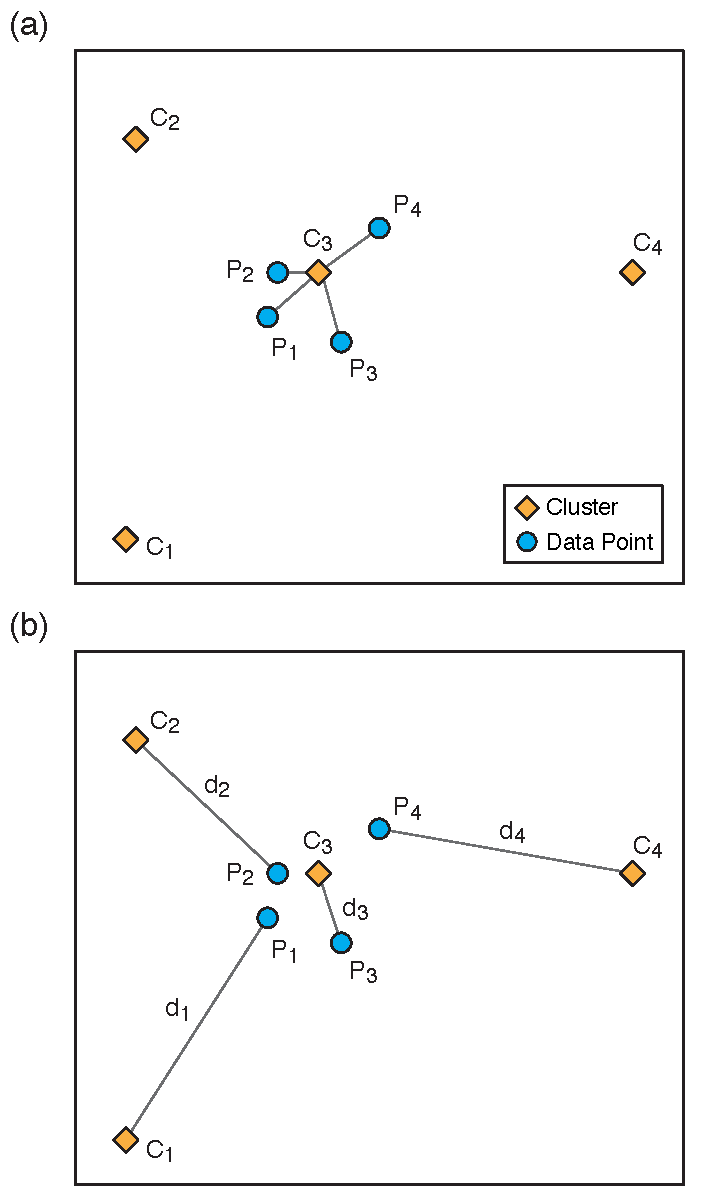
\includegraphics[width=\columnwidth]{figures/pdf/figure-04}
	\caption{Representation of the (a) ordinary, and (b) constrained \kmeans{} approaches for four data-points (P) and four cluster centers (C) in a 2D dataset space, where all the data-points are constrained to be cannot-link points. The color version of this figure is available only in the electronic edition.}
	\label{fig:k-means}
\end{figure}

This process is sensitive to the initial selection of the clusters and their centers. To mitigate this, constrained \kmeans{} introduces two types of constraints: must-link and cannot-link \citep{Wagstaff_2001_Proc}. The must-link constraint specifies instances in which two data-points must be linked, i.e., in the same cluster. The cannot-link constraint specifies instances in which data cannot be in the same cluster. This prevents the process from converging into a local minimum, and defines constrained \kmeans{} as a semi-supervised method. Figure \ref{fig:k-means} illustrates the differences between the standard and constrained \kmeans{} methods for a single clustering iteration on a small two-dimensional dataset.

In our implementation we limit the clustering to four validation categories: poor, fair, good, and excellent. The cluster centers are randomly selected at the start, but we apply constraints by adding 4 artificial stations with cannot-link conditions that are checked at the end of each iteration. These stations are associated with each type of cluster and have GOF scores equal to 3, 5, 7, and 9, across all metrics, thus they are representative of the validation categories. 

In the multi-dimensional space defined by the 11 GOF metrics used here, the distances are obtained using the Euclidean expression:
% 
\begin{equation}
	d(x_i, x_j) = \sqrt{ \sum_{l=1}^{n} \left( x_{i,l} - x_{j,l} \right)^2 } 
\end{equation}
% 
corresponding to the distance $d$ between the data-point $x_i$ and the cluster center $x_j$ in the $n$-dimensional domain, where $x_{i,l}$ is the $l$-th feature of the data-point $x_i$, and $x_{j,l}$ is the $l$-th feature of the cluster center $x_j$. It is, however, unpractical to expect the patterns defining the clusters to be observable across all features. Such high-dimensional issues are well known \citep[see, for instance,][]{Parsons_2004_ACM, Dy_2004_MLR}, and can be tackled using sub-spaces. Therefore, instead of analyzing all $2^{11}$ possible sub-spaces, we focus only on sub-spaces with 2, 3, and 4 dimensions, or features. In total, we analyze 550 sub-spaces, 55 sub-spaces with 2 features, 165 with 3, and 330 with 4.

Unfortunately, not all the sub-spaces will have clearly distinguishable clusters (i.e., some will not satisfy the cannot-link constraints even after a large number of iterations). Such sub-spaces are discarded, and all others are used to label the data. In an ideal case, each station will be labeled 550 times, and the final label is taken as the mode. For example, if after all the sub-spaces are accounted for, a station has labels $\left\{F, F, F, P, F, G, E, F, F\right\}$, where the labels $P$, $F$, $G$, and $E$ correspond to the poor, fair, good, and excellent category clusters, then such as station will be given a final label $F$. Once all the data is properly labeled, we proceed with the decision tree analysis.


% ===========================================================================================
%


% Although we do not expect to see the pattern that resulted from clustering using 11 features in presentation of only two, however, different studies show that the higher dimension reduce the effect of similarity based on distance. \citet{Parsons_2004_ACM} presented an illustrative example to show the effect of dimension in reducing the importance of the distance. Effect of higher dimensions in clustering has been well studied and many different methods are proposed to reduce this effect in the final results. Among them we can name  feature selection before, during, and after clustering, hybrid methods that use combination of methods to select the best subset of feature. \citet{Dy_2004_MLR} addressed two issues involved in developing an automated feature subset selection algorithm for unlabeled data. They illustrated the irrelevant and redundant features and proposed methods for evaluating candidate features using two performance criteria.

% Subspace analysis is another technique to address the challenges with higher dimensional data in clustering process. Subspace clustering is an extension of traditional clustering which looks for different pattern using subset of features.  \citet{Parsons_2004_ACM} provided a list of algorithm for conducting subspace clustering and also some potential applications for them. The most common factor among these algorithm is the process to find a group of best subspaces through optimization process. An n-dimensional dataset has $2^n$ subspaces where it could be very costly and time consuming to evaluate all of them.

% In this study we are interested in using those features who, in general, represent the simulation accuracy in 4 different categories. As a first step we use the constrained \kmeans{} clustering approach for all features, however, because of mentioned reasons the results are not easy to discuss or even evaluate. Although we have four groups of data, the question is which one should be considered as poor, fair, good, or excellent groups. Therefore, we apply a modified method of subspace clustering approach to cluster the stations. As we discussed earlier and presented in figures the constrained \kmeans{} method effectively put the stations in a cluster with considering the fact that our constrain stations should not be in the same cluster. High number of iteration leads the clustering process to follow the clustering concept that we are looking for which is clustering stations as poor, fair, good, and excellent. In our case number of possible subspace is $2^{11}$ where each features have two options wether belong to subspace or not. However, because of preserving the distance based criteria effects we limited the number of features in the subspace to be 2,3, and 4 features. Therefor we have 330,165, and 55 unique subspaces for 4D,3D, and 2D, respectively. We conduct a constrained \kmeans{} clustering analysis for each of these subspaces and repeat the algorithm. In some cases, it is not possible to distinguish all four cannot-link stations in different clusters. In this study we ignore these cases. We only use those combination of features that gives 4 unique clusters for the constraint points (hypothetical stations), therefore, we know for sure that all data within same cluster let's say with metric value 3, should be considered as poor. We also control the clusters to be consistent (we reformat numbers to assign cluster 1 to all group of stations that our first constraint belongs to them and so on). Finally, using 550 unique subspace clustering results, we assign the most frequent class to the station.





% and computes . These distances are then used as a criteria to determine the cluster to which cluster each data-point belongs. 

% ...


% \citet{Macqueen_1967_Proc} describes this method as a process for partitioning a $n$-dimensional population into $k$ sets on the basis of a sample. Its algorithm produces partitions that are reasonably efficient in the sense of within-class variance. It starts with a user defined number of clusters ($k$) and assigns a random mean value to each cluster (or randomly choose $k$ data-points and assigns them as cluster centers). After this, the algorithm computes the distances of all other data-points to the center of the cluster and uses the distance as a criteria to clustering the data points. Because the data resides in a multi-dimensional space (here defined by each metric), there are different ways of computing the distance of each data-point to the cluster's center. We use the Euclidean distance:
% % 
% \begin{equation}
% 	d(x_i, x_j) = \sqrt{ \sum_{k=1}^{n} \left( x_{i,k} - x_{j,k} \right)^2 } 
% 	\, ,
% \end{equation}
% % 
% where $n$ is the number of features and $d$ is the distance of $x_i$ and $x_j$ in $n$-$dimensional$ domain. 




% ===========================================================================================
%
% NEW TEXT PROVIDED BY NAEEM ON JAN 22
% Once the distance is computed, the algorithms labels the data based on the proximity of each point to each cluster, and computes the arithmetic mean value of the data for each cluster, and assigne that value as the updated location of each cluster's center. The algorithm repeats the steps unless the amount of updates among the cluster centers is less than a predefined tolerance value. The major problem with \kmeans{} algorithm is that it is sensitive to the selection of the initial partition and may converge to a local minimum of the criterion function value if the initial partition is not properly chosen. Another problem accompanying the use of \kmeans{} algorithm is the choice of the number of desired output clusters. \citep{Jain_1999_ACMCS}. Clustering is a subjective process. The same set of data items often needs to be partitioned differently for different application. In our application the number of clusters according to the literature is 4 (i.e., poor, fair, good, and excellent.) However, our initial attempts represents that the results are highly sensitive to the initial clusters' center. Therefore, we need to incorporate the experts knowlege in the process. 


% \citet{Wagstaff_2001_Proc}  demonstrated a modification of \kmeans{} clustering algorithm which uses the background information of the domain or dataset. The algorithm adds two types of constraints to the clustering including:
% 	% 
% 	\begin{itemize}
% 	\item{Must-link: constraints specify that two instances have to be in the same cluster.}
% 	\item{Cannot-link: constraints specify that two instance must not be placed in the same cluster.}
% 	\end{itemize} 
% 	% 
% The algorithm is described in detail in \citet{Wagstaff_2001_Proc}, however, in simple words, in the ordinary \kmeans{} process before assigning data to the closes cluster, it controls the must-link and cannot-link conditions. Therefore, in this case, the closest cluster's center is not necessarily the final cluster of the data.


% In a hypothetical assumption, if we have a pair of data and synthetic with GOF score of 3 for all metrics we could consider the overall simulation GOF as poor. This is also correct for 5,7, and 9 that we can assigne them fair, good, and excellent class, respectively. Therefore, we add 4 hypothetical stations into the dataset with GOF score of 3,5,7,and 9 for all metrics and we put them in cannot-link constraint. This assumption that originated from the experts knowledge, provides enough information to the algorithm to converge to the same final clusters and cluster centers after a reasonable amount of iteration. 

% Fig.~\ref{fig:con_kmeans} presents the difference between ordinary and constrained k-means clustering approach using 4 points and 4 cluster centers. Fig.~\ref{fig:con_kmeans}.a presents the \kmeans{} without constrained. According to the definition and the explanation in this section, the closest cluster center for each points will get the points. 	Fig.~\ref{fig:con_kmeans}.b represents the constrained \kmeans{} approach, where, the closest cluster center is not necessarily the final cluster. The data points can not be in the same cluster, in result,  we assign them to different clusters in this case to satisfy the Cannot-link criteria. The best configuration happens when we minimize the distance between cluster centers and points.

% ===========================================================================================
% 
% OLD STUFF DONE BY RICARDO FOR THE INTRO OF THIS SECTION
% 
% In machine learning, decision trees are classified as a supervised learning method, and the first step towards designing them requires that the data be labeled according to their attributes. The inherent attribute of our data are the GOF value themselves, but because of the multiplicity of metrics and the lack of clarity about how these relate to each other, we need to add labels to the data that are in accordance with the outcome attributes, i.e., in terms of the predefined validation quality levels. We label the data in our dataset by means of a clustering process. 

% There exist different methods for clustering data \citep[see Chapters 10 and 11 in][]{Han_2011_Book}, among which the \kmeans{} and constrained \kmeans{} clustering methods are the most widely used \citep{Jain_1999_ACMCS}. We note about these methods that the \kmeans{} approach is sensitive to the initial values chosen to be at the center of the clusters---especially in the case of data that are not clearly distinguishable---, whereas the constrained \kmeans{} method uses background knowledge to overcome this limitation. Because of its use of background information, the modified \kmeans{} method is considered as a semi-supervised process.





% ===========================================================================================
%
% SECOND ATTEMPT THAT WAS RECALLED BY NAEEM

% Once the distance is computed, the algorithms labels the data based on the proximity of each point to each cluster, computes the mean value of the data for each cluster, and updates the location of each cluster's center. \textcolor{red}{(How do we compute ``mean value'' and how do we recompute the ``center''? All what follows after this in the original text is too descriptive, and not specific enough. We need to go to the point and this is going in long description circles.)} 

% {\color{gray}
% 	The algorithm repeats the steps unless the amount of updates among the cluster centers is less than a tolerance value.  \kmeans{} clustering has been applied in different applications, however, there is no clustering technique that is universally applicable in uncovering the variety of structures present in multidimensional datasets. Therefore, clustering is a subjective process. The same set of data items often needs to be partitioned differently for different application. In result, it is essential for the user of a clustering algorithm to not only have a thorough understanding of the particular technique being utilized, but also to know the details of the data gathering process and to have some domain expertise; the more information the user has about the data at hand, the more likely the algorithm would be able to succeed in assessing its true class structure. Domain concept can play several roles in the clustering process, and a variety of choices are available to the practitioner \citep{Jain_1999_ACMCS}. 

% 	The major problem with \kmeans{} algorithm is that it is sensitive to the selection of the initial partition and may converge to a local minimum of the criterion function value if the initial partition is not properly chosen. Another problem accompanying the use of \kmeans{} algorithm is the choice of the number of desired output clusters. Several variant of the \kmeans{} algorithm have been reported in the literature. Some of them attempt to select a good initial partition so that the algorithm is more likely to find the global minimum value, another variation is to permit splitting and merging of the resulting clusters \citep{Jain_1999_ACMCS}. 

% 	In our application the number of clusters is not a problem and there is a consensus among researchers in the number of clusters (i.e., poor, fair, good, excellent), however, our initial attempts represent that the results are highly sensitive to the initial clusters' center. 

% 	Every clustering algorithm uses some type of knowledge either implicitly or explicitly. In this study the background knowledge is a series of hypothetical stations. We assume that there are four stations with score of 3, 5, 7, and 9 for all of their metrics. Based on the score limits in section.~\ref{validation_metrics} we know these stations belong to poor, fair, good, and excellent classes, respectively. These background knowledge could help the clustering processing to be in right direction regarding the fact that increasing dimension of data could increase noise in clustering and cause difficulty to better partitioning. \citet{Wagstaff_2001_Proc}  demonstrated a modification of \kmeans{} clustering algorithm which uses the background information of the domain or dataset. The algorithm adds two types of constraints to the clustering including:
% 	% 
% 	\begin{itemize}
% 	\item{Must-link: constraints specify that two instances have to be in the same cluster.}
% 	\item{Cannot-link: constraints specify that two instance must not be placed in the same cluster.}
% 	\end{itemize} 
% 	% 
% 	The algorithm is described in detail in \citet{Wagstaff_2001_Proc}, however, in simple words, in the ordinary \kmeans{} process before assigning data to the closes cluster, it controls the must-link and cannot-link conditions. Therefore, in this case, the closest cluster's center is not necessarily the final cluster of the data. Fig.~\ref{fig:con_kmeans} presents the difference between ordinary and constrained k-means clustering approach using 4 points and 4 cluster centers. Fig.~\ref{fig:con_kmeans}.a presents the \kmeans{} without constrained. According to the definition and the explanation in this section, the closest cluster center for each points will get the points.
	
% 	Fig.~\ref{fig:con_kmeans}.b represents the constrained \kmeans{} approach, where, the closest cluster center is not necessarily the final cluster. The data points can not be in the same cluster, in result,  we assign them to different clusters in this case to satisfy the Cannot-link criteria. The best configuration happens when we minimize the distance between cluster centers and points. Using this method at each step the algorithm redistribute the 4 hypothetical stations to satisfy the cannot-link constraint. The visual inspection of the figures also confirms the accuracy of the method. Doing this, in the next iteration this data manipulation leads the cluster center in a direction to have the hypothetical station in the cluster and loose those data that is in far other side direction of the hypothetical station. Therefore, the cluster tend to have all data that similar to the hypothetical station. \\
% 	The end product of the clustering process is groups of data. Analysis of these groups, individually, gives the idea about the clusters in terms of within class variation. In these analysis we mainly study the behavior of different features in each cluster and isolate only the most descriptive features to be used in the supervised classifier that assumes a given number of classes in the data set. In the next section we provide a basics of decision tree algorithm. 

% }

% In other words, the points cannot be in the same cluster. In the constrained \kmeans{} approach we redistribute the points such that the $\sum{d}$ becomes minimum.

% ===========================================================================================
%
% OLD NAEEM VERSION
% 
% Clustering is an unsupervised approach for grouping of data based on measure of similarity and it is considered as an exploratory activity as a part of data mining process \citep{Fayyad_1996_IEEE}. In each valid cluster, patterns are more similar in each other than they are to pattern belonging to a different cluster. Many clustering algorithms are developed for different application, however, study the difference of them is beyond the scope of this paper. In general, at the top level,  \citet{Jain_1999} distinguished the clustering approach into Hierarchical and Partitional approaches. Aside from differences in application and technical details in implementation, hierarchical methods produce nested series of partitions, while partitional methods produce only one. In this study we are interested in using partitional, distance based clustering algorithm, which is also known as \kmeans{} algorithm.  \citet{Macqueen_1967_Proc}  described a process for partitioning an $n$-$dimensional$ population into $k$ sets on the basis of a sample. The process appears to give partitions which are reasonably efficient in the sense of within-class variance. For numerical values, \kmeans{} algorithm starts with a user defined number of clusters (k) and assign a random mean value for each cluster (or randomly choose k data and assign them as cluster centers.) Then it computes the distance of data and cluster centers. A variety of distance measures are in use in different studies, however, we use the Euclidean distance through 

% \begin{equation}
% d(x_i,x_j)=\sqrt{\Sigma_{k=1}^{n}(x_{i,k} - x_{j,k})^2},
% \end{equation}

% where $n$ is the number of features and $d$ is the distance of $x_i$ and $x_j$ in $n$-$dimensional$ domain. After computing the distance of the points from each clusters' mean (center), the algorithm continues with labeling the data after the closest cluster. At the next iteration, it computes the mean value of data for each cluster and updates the clusters' centers. The algorithm repeats the steps unless the amount of updates among the cluster centers is less than a tolerance value.  \kmeans{} clustering has been applied in different applications, however, there is no clustering technique that is universally applicable in uncovering the variety of structures present in multidimensional datasets. Therefore, clustering is a subjective process. The same set of data items often needs to be partitioned differently for different application. In result, it is essential for the user of a clustering algorithm to not only have a thorough understanding of the particular technique being utilized, but also to know the details of the data gathering process and to have some domain expertise; the more information the user has about the data at hand, the more likely the algorithm would be able to succeed in assessing its true class structure. Domain concept can play several roles in the clustering process, and a variety of choices are available to the practitioner \citep{Jain_1999}. 

% The major problem with \kmeans{} algorithm is that it is sensitive to the selection of the initial partition and may converge to a local minimum of the criterion function value if the initial partition is not properly chosen. Another problem accompanying the use of \kmeans{} algorithm is the choice of the number of desired output clusters. Several variant of the \kmeans{} algorithm have been reported in the literature. Some of them attempt to select a good initial partition so that the algorithm is more likely to find the global minimum value, another variation is to permit splitting and merging of the resulting clusters \citep{Jain_1999}. 

% In our application the number of clusters is not a problem and there is a consensus among researchers in the number of clusters (i.e., poor, fair, good, excellent), however, our initial attempts represent that the results are highly sensitive to the initial clusters' center. 

% Every clustering algorithm uses some type of knowledge either implicitly or explicitly. In this study the background knowledge is a series of hypothetical stations. We assume that there are four stations with score of 3, 5, 7, and 9 for all of their metrics. Based on the score limits in section.~\ref{validation_metrics} we know these stations belong to poor, fair, good, and excellent classes, respectively. These background knowledge could help the clustering processing to be in right direction regarding the fact that increasing dimension of data could increase noise in clustering and cause difficulty to better partitioning. \citet{Wagstaff_2001_Proc}  demonstrated a modification of \kmeans{} clustering algorithm which uses the background information of the domain or dataset. The algorithm adds two types of constraints to the clustering including:\\
% \begin{itemize}
% \item{Must-link: constraints specify that two instances have to be in the same cluster.}
% \item{Cannot-link: constraints specify that two instance must not be placed in the same cluster.}
% \end{itemize} 
% The algorithm is described in detail in \citet{Wagstaff_2001_Proc}, however, in simple words, in the ordinary \kmeans{} process before assigning data to the closes cluster, it controls the must-link and cannot-link conditions. Therefore, in this case, the closest cluster's center is not necessarily the final cluster of the data. Fig.~\ref{fig:con_kmeans} presents the difference between ordinary and constrained k-means clustering approach using 4 points and 4 cluster centers. Fig.~\ref{fig:con_kmeans}.a presents the \kmeans{} without constrained. According to the definition and the explanation in this section, the closest cluster center for each points will get the points.
% Fig.~\ref{fig:con_kmeans}.b represents the constrained \kmeans{} approach, where, the closest cluster center is not necessarily the final cluster. The data points can not be in the same cluster, in result,  we assign them to different clusters in this case to satisfy the Cannot-link criteria. The best configuration happens when we minimize the distance between cluster centers and points. Using this method at each step the algorithm redistribute the 4 hypothetical stations to satisfy the cannot-link constraint. The visual inspection of the figures also confirms the accuracy of the method. Doing this, in the next iteration this data manipulation leads the cluster center in a direction to have the hypothetical station in the cluster and loose those data that is in far other side direction of the hypothetical station. Therefore, the cluster tend to have all data that similar to the hypothetical station. \\
% The end product of the clustering process is groups of data. Analysis of these groups, individually, gives the idea about the clusters in terms of within class variation. In these analysis we mainly study the behavior of different features in each cluster and isolate only the most descriptive features to be used in the supervised classifier that assumes a given number of classes in the data set. In the next section we provide a basics of decision tree algorithm. 


% \begin{figure}
%     \centering
%     \includegraphics
%       %  [width=\columnwidth]
%         [width=200px]
%         {figures/pdf/Figure_4.pdf}
%     \caption{ Representation of ordinary (a) and constrained (b) \kmeans{} approach. There are four data points (p) and four cluster centers (c) as a sample of $2$-$Dimensional$ dataset. All points are defined as cannot-link constraints. In other words, the points cannot be in the same cluster. In the constrained \kmeans{} approach we redistribute the points such that the $\sum{d}$ becomes minimum.}
%     \label{fig:con_kmeans}
% \end{figure}


% 
Decision tree learning is a method for approximating a target function, in which learned function is represented by decision tree \citep{Mitchell_1997_Book}. \citet{Quinlan_1986} demonstrated that the technology for building decision trees from examples is fairly robust. He summarized an approach to synthesizing decision trees that has been used in a variety of systems, and he describes one such system, ID3, in detail. Although ID3 algorithm is successful in most classification problems, it does not handle the numeric attributes and only one attribute at a time is tested for making decisions. \citet{Quinlan_1993} extended the ID3 algorithm and presented the C4.5 algorithm. Later on they added boosting capability to C4.5 and called it C5.0. The improved algorithm accepts both continues and discrete features and solves over fitting problem by pruning. Although there are many other algorithm for implementing decision tree, in this study we use the C5.0 algorithm. Discussing the algorithm in details is out of the scope of this paper. There are fairly good amount of references to study those details \citep[e.g.,][]{Mitchell_1997_Book,Quinlan_1993,Hornik_2009}.\\
In general, decision tree measures the effectiveness of an attribute in classifying the training data through information gain. According to  \citet{Mitchell_1997_Book}, information gain of an attribute is the expected reduction in entropy caused by partitioning the examples according to this attribute. If the target can take on $c$ different values the entropy is defined as
\begin{equation}
Entropy(S) = \sum_{i=1}^{c} -p_{i}\ log_2\ p_i,
\end{equation}

where $p_i$ is proportion of $S$ belonging to class $i$. Entropy measures the homogeneity of examples or dataset. Higher entropy means data is  fairly uniformly distributed among different classes. On the other hand lower entropy means data unequally distributed among classes. The extreme case happens when all data belong to one class which results in entropy equal to zero. Given entropy as a measure of impurity in a collection of training example the measure of the effectiveness of attribute is defined through information gain which is expected reduction in entropy caused by partitioning the examples according to this attribute. Gain of the attribute A is defined as 

\begin{equation}
Gain(S,A)\ =\ Entropy(S) - \sum_{v \in Values(A) } \frac{|S_v|}{|S|} Entropy(S_v)
\end{equation} 

where $Values(A)$ is the set of all possible values of attribute A, and $S_v$ is the subset of $S$ for which attribute $A$ has value $v$. Information gain is used by the algorithm in order to determine which is the better attribute for classifying the training example. The attribute with higher information gain will be the first option to separate the training data based on and grow to the lower nodes ( For more detailed examples refer to chapter 3 of \citet{Mitchell_1997_Book}). \\
We discussed the basic idea behind the decision tree algorithm, however, there are more details specially in dealing with outliers and noises which we address them through pruning approaches. In this study we use C5.0 package \citep{C50_2015} in R to conduct the decision tree algorithm. We discuss the input parameters in the section.\ref{classification_model}.  

% More text for use
%========================= \\
 %The method uses background knowledge to direct the clustering in an appropriate direction so the results are close to real data. Obviously there will be some features that is not obey the general pattern among these features. We will put aside those features. Then we try to modify those features to be able to use again in the processing. In the other words we will scale those features to obey the general trend. Anderson(2004) divided the stations into four main groups based on those stations scores. In hypothetical case were two signals are identical these scores should be 10. However, if they are not the same, but the scoring method provides similar results we should get a fairly close score for all matrics. In real cases the scores are different from one another. However, if we could define a metrics that gives a similar level of goodness of fit for all of them then we can for sure categorized the station in an appropriate group. In this study we define 4 hypothetical stations with score of 3,5,7, and 9 which represent middle points for poor, fair, good and excellent goodness of fit categories. Any station close to these stations should reflect the idea that they are at the same group. However, they are slightly different and we want to know why and how we can make them similar. So having these hypothetical stations and forcing the constrained k-means algorithm to put these stations in different groups we are able to bring the background knowledge into the process. So in the study we start with one attribute and cluster stations. According to figures (2D and 3D) we can argue that the background knowledge assisted the k-means clustering to cluster the stations, realistically. Meanwhile it could not force the clusters to have a cluster centers as those points.  We assign the most frequent stations' cluster to that station. Then we study the score variation in each group and see if they have a uniform behavior if not we can further study the potential problems with that score and probable scaling factors to make it obey the pattern. We also analyze the effect of velocity model, earthquake, orientation, frequency band in the final results. 
%Based on having class for each station in the study we develop a decisition tree to provide the group of simulation for Los Angles Basin earthquakes.  \\

%To do list: \\

%Another approach to go is considering all data without separating for earthquake, velocity model, and so on. Then try to put them in one cluster. Those stations which are in the cluster but are in extreme case, remove from the data base. \\
%Analyze inside each cluster, provide normal distribution, if data looks ok keep it, if not remove those features. \\
%Normally majority of dimensions are irrelevant in high dimensional data. These irrelevant dimensions can hide clusters in noisy data and confuse the clustering algorithm. \\
%Try different method and cluster data, then find the points that clustered currently then use that points as a must link condition. \\
%We can not show data with 10 attributes in graph, however, we can generate a set of statistical figures of changing these values in the figure.\\ 
%If using a feature cause to not able to fit the station in any class we remove it or give a factor to put in the right class.\\
%in the end we want to have all stations as constrained. In other word, we start from 1D and if there is a station that is always in the same group we added it in constraint points. then we move to the 2D and we continue the same until we have all station as constraint.\\
%Constraint helps the clustering to get the same results after good amount of iterations.\\
%========================= \\

% 
\section{Clustering Analysis}

We start with clustering all dataset with 11 features. Visual presentation of results above 3 dimension is not possible. Therefor we present the clustering results based on a pair of features in Fig.~\ref{fig:CxCy_11}. 
\begin{figure}
    \centering
    \includegraphics
       % [width=\columnwidth]
        [width=\textwidth]
        {figures/pdf/Figure_5.pdf}
    \caption{Results of clustering analysis with all 11 attributes (metrics). This results are subsample of 55 possible combination of metrics. Center of cluster is shown as crosses. At this plot ordinal, categorical clusters' numbers are not necessarily represent the poor, fair, good, and excellent. }
    \label{fig:CxCy_11}
\end{figure}
The figure represent a part of results in clustering with 11 features. There are 55 other possibility to present (e.g., C1 vs C7 or C2 vs C9). As one can see in some combination of features the clustering patterns are easily seen. For example in C3 vs C4 we can distinguish 4 region for clusters, although they are partly mixed together. This also correct for C6 vs C7 and C7 vs C8. In the latter one we observe less mixture of data than the former one. Also there are other types of figures where one feature does not add so much information to the clustering process. For example in C9 vs C10, C10 could be considered as irrelevant feature. Irrelevant feature does not add further information for clustering and redundant feature add the equivalent information as other feature \citep{Dy_2004_MLR}. The last combination of features are a good mixture of data and it is not possible to see the clustering boundaries. C1 vs C2 and C10 vs C11 are examples of such feature combination. It is worth to mention that at this point the cluster numbers are not consistent with ordinal categorical numbers of 1,2,3, and 4 representing poor, fair, good, and excellent, respectively.\\   
Although we don't expect to see the pattern that resulted from clustering using 11 features in presentation of only two, however, different studies show that the higher dimension reduce the effect of similarity based on distance. \citet{Parsons_2004_ACM} presented an illustrative example to show the effect of dimension in reducing the importance of the distance. Effect of higher dimensions in clustering has been well studied and many different methods are proposed to reduce this effect. Among them we can name  feature selection before, during, and after clustering, hybrid methods that use combination of methods to select the best subset of feature and subspace analysis. \citet{Dy_2004_MLR} addressed two issues involved in developing an automated feature subset selection algorithm for unlabeled data. They illustrated the irrelevant and redundant features and proposed methods for evaluating candidate features using two performance criteria. \\
Subspace analysis is another technique to address the challenges with higher dimensional data in clustering process. Subspace clustering is an extension of traditional clustering which looks for different pattern using subset of features.  \citet{Parsons_2004_ACM} provided a list of algorithm for conducting subspace clustering and also some potential applications for them. The most common factor among these algorithm is the process to find the a group of best subspaces through optimization process. An n-dimensional dataset has $2^n$ subspaces where it could be very costly and time consuming to evaluate all of them.\\
As we discussed earlier, there is not standard measures for evaluating clusters in the clustering literature also there is no single clustering assignment explains every application \citep{Dy_2004_MLR,Jain_1988_Book,Hartigan_1985_JOC}. The clustering process is strongly dependent on the application. A good example of the concept is clustering a whale, an elephant, and a tuna fish \citep{Jain_1999,Watanabe_1985_Book}.  Whales and elephants should be in the same cluster, because they both are mammals. However, regarding the scope of the clustering the user could put tuna fish and whales in the same cluster because both groups live in water. In this study we are interested in using those features who, in general, represent the simulation accuracy in 4 different categories. As a first step we used the \kmeans{} clustering approach for all features, however, because of mentioned reasons the results are not easy to discuss or even evaluate. Although we have four groups of data, the question is which one should be considered as poor, fair, good, or excellent groups. Therefore, we apply a modified method of subspace clustering approach to cluster the stations. As we discussed earlier and presented in figures the constrained \kmeans{} method effectively put the stations in a cluster with considering the fact that our constrain stations should not be in the same cluster. High number of iteration leads the clustering process to follow the clustering concept that we are looking for which is clustering stations as poor, fair, good, and excellent. In our case number of possible subspace is $2^{11}$ where each features have two options wether belong to subspace or not. However, because of preserving the distance based criteria effects we limited the number of features in the subspace to be 2,3, and 4 features. Therefor we have 330,165, and 55 unique subspaces for 4D,3D, and 2D, respectively. We conduct a \kmeans{} clustering analysis for each of these subspaces. After considering the constraint conditions, which is assigning cannot-link stations to different cluster and and repeat the \kmeans{} algorithm, in some cases, it is not possible to distinguish all four cannot-link stations in different clusters. In this study we ignore these cases. We only use those combination of features that gives 4 unique clusters for the constraint points (hypothetical stations), therefore, we know for sure that all data within same cluster let's say with metric value 3, should be considered as poor. We also control the clusters to be consistent (we reformat numbers to assign cluster 1 to all group of stations that our first constraint belongs to them and so on). Finally, using 550 unique subspace clustering results, we assign the most frequent class to the station. 


Fig.~\ref{fig:C_cvm_comp} shows the results for different velocity models and components. A preliminary visually inspection shows that the behavior of scores with respect to the velocity model is similar. Therefor we merge data of different velocity models.  Fig.~\ref{fig:Figure_cluster_comp} shows the results. 

\begin{figure}
    \centering
    \includegraphics
       % [width=\columnwidth]
        [width=\textwidth]
        {figures/pdf/Figure_6.pdf}
    \caption{Box plot of data used in the study. Metrics shown for C1 to C11 for 3 components in separate plots for velocity models and clusters. Median of data are shown as a notch. Thick lines represent the IQR (Interquartile Range, Q3-Q1) of data. Outliers (data less than Q1-1.5*IQR and greater than Q3+1.5*IQR) are shown as scatter dots above and below plots if applicable.}
    \label{fig:C_cvm_comp}
\end{figure}

\begin{figure}
    \centering
    \includegraphics
       % [width=\columnwidth]
        [width=\textwidth]
        {figures/pdf/Figure_7.pdf}
    \caption{Box plot of data used in the study. Metrics shown for C1 to C11 for 3 components in separate plots for  clusters. Median of data are shown as a notch. Thick lines represent the IQR (Interquartile Range, Q3-Q1) of data. Outliers (data less than Q1-1.5*IQR and greater than Q3+1.5*IQR) are shown as scatter dots above and below plots if applicable.}
    \label{fig:Figure_cluster_comp}
\end{figure}

Although there are some differences in the scores based on different components, there are general similarity in all clusters for different metrics among their components. Fig.~\ref{fig:Figure_cluster_all_comp} shows the results with merging the components. 


\begin{figure}
    \centering
    \includegraphics
       % [width=\columnwidth]
        [width=\textwidth]
        {figures/pdf/Figure_8.pdf}
    \caption{Box plot of data used in the study. Metrics shown for C1 to C11  in separate plots for  clusters. Median of data are shown as a notch. Thick lines represent the IQR (Interquartile Range, Q3-Q1) of data. Outliers (data less than Q1-1.5*IQR and greater than Q3+1.5*IQR) are shown as scatter dots above and below plots if applicable.}
    \label{fig:Figure_cluster_all_comp}
\end{figure}

Fig.~\ref{fig:Figure_cluster_all_comp} represents the results from a broad perspective. It is necessary to do statistical significance tests to understand the effect of component, velocity model, earthquake, and frequency band in the results.  According to Fig.~\ref{fig:Figure_cluster_all_comp} scores C1, C2, and C11 has the least changes in different clusters. They suggest the idea that they may not helpful in defining a decision rule. On the other hand, other scores are fairly variable among different clusters. 
Scores C1, C2, and C10 are very similar in cluster 1 to 3. However, we can see a small increase in cluster 4 for these scores. Also the data variation becomes small and range of data moves higher. Scores C3-C9 have a considerable increment from cluster 1 to cluster 4. Although there are a broad variation of data in cluster 3 and cluster 4 for these scores, good amount of data (50\% based on the IQR) are in a small range and increasing with respect to the clusters. C11 has a constant behavior with a small reduction in median at cluster 4. Fig.~\ref{fig:Figure_cluster_barplot} shows number of stations in each cluster based on component. 

\begin{figure}
    \centering
    \includegraphics
       % [width=\columnwidth]
        [width=300px]
        {figures/pdf/Figure_9.pdf}
    \caption{Number of data in each cluster based on components after conducting constraint \kmeans{} clustering through subspace analysis.}
    \label{fig:Figure_cluster_barplot}
\end{figure}





\section{Classification model} \label{classification_model}

In the section.~\ref{methodology} we discussed the basics of decision tree method and we provided a brief history of available algorithm. In this section we develop a classification model. Although there are numerous methods to classify labeled data, however, in this study we are interested in a method to not only predict the class of simulation based on metrics, but also give an intuition about the decision process. Therefor we use tree based algorithm to develop the prediction model.\\

After preprocessing data the most important step in developing a prediction model is feature selection. The step becomes more relevant when data set has hundreds to tens of thousands of variable or features. Although our dataset does not have numerous features we do some analysis on features before developing the prediction model. Features of a dataset could have similar behavior. This characteristic is easy to understand by correlation criteria. The Pearson correlation coefficient between two features is defined as

\begin{equation}
R(i)=\frac{cov(X_i,X_j)}{\sqrt{var(X_i)var(X_j)}},
\end{equation} 

where $cov$ is covariance function and $var$ is the variance function \citep{Guyon_2003}. Fig.~\ref{fig:Corplot} represent the Pearson Correlation factor among features.  

\begin{figure}
    \centering
    \includegraphics
       % [width=\columnwidth]
        [width=200px]
        {figures/pdf/Figure_10.pdf}
    \caption{Pearson correlation values between metrics. The plot is generated using Corrplot package in R \citep{Corrplot_2016}}
    \label{fig:Corplot}
\end{figure}

As we can see from the figure some metrics are highly correlated. Among them we can mention C1 vs C2 , C3 vs C4, C5 vs C6 and C8, and C6 vs C8 have correlation factor more than 90\%. Also we observe that C11 is mostly have a negative correlation with other features. Feature selection is a broad research field. \citet{Guyon_2003} presented a review of common methods to select features, construct new features or reduce the domain. They highlighted the fact that redundant variable or variables that are useless by themselves may be useful in combination with other variables. Clustering is a method to construct new features as an unsupervised learning or feature selection without having the labels in calculation. The idea is to replace a group of features mean with newly developed features. It helps to reduce the number of features and use all of the available information \citep{Duda_1973,Guyon_2003}. Since we don't have a long list of features and also we want to study all feature effects we leave all features to be used in the prediction model. 

After analysis of each features the next step is subsetting data for training and testing process. A subset of data that is used for training and test should have about the equal distribution of target values. Equally distributed data helps training process to not biased to an special class also helps to have an accurate evaluation of the model during the test process. Imbalanced data may decrease the classifier performance. A dataset is imbalanced if the classification categories are not approximately equally represented. \citet{Branco_2015} provided a comprehensive review of different approaches toward imbalanced distribution of target variables. A mostly common approach is data preprocessing through resampling. According to \citet{Branco_2015}, resampling strategies based on diverse set of techniques such as: random under/over-sampling, distance methods, data cleaning approaches, clustering algorithm among them.\\
According to the clustering results, among all data with different components and velocity model there are 816,1253,879, and 76 data belong to cluster 1,2,3, and 4, respectively. \citet{Weiss_2003} discussed the fact that the perfectly balanced dataset does not always provide the optimal results. One option could be under sampling cluster 1 to 3 to be in the similar distribution of cluster 4. This may eliminate the useful examples leading to a worse performance. Therefor we 10 times over-sample the data with cluster 4 to have a distribution similar to other cluster. Oversampling may increase the likelihood of overfitting, however, in this case the oversampling rate is not high. On the other hand, using pruning method during training as well as evaluating algorithm with unseen test dataset we address the overfitting issue.  Choosing what fraction of data should be used for training and testing is an open question. We put 30 percent of data for test and 70 percent of data for training. 

Different measures are defined for evaluation of performance of prediction models. Two main metrics are precision and recall. In a simple word, in a binary case, precision represent the fact that how many of predicted values as positive is actually positive and recall represent the idea that how many of positive cases are diagnosticated with the algorithm. Choosing between these two measures is dependent on the application. For example if there is a highly contagious disease and we want to put all contaminated persons in a quarantine, we need to focus on recall value, because even if we miss one case, it could distribute the virus, however, there is a trade off between recall and precision. In the mentioned example there should be some person that indicated as contaminated with virus where as they are not. Therefor, the algorithm precision is not high. Table~\ref{tab:confusion_def} which is called confusion matrix is a method to represent the overall functionality of the algorithm \citep{Branco_2015}.  


\begin{table}
\centering
\caption{Confusion Matrix for binary problem}
\label{my-label}
\begin{tabular}{llll}
\hline
                                                 &                              & \multicolumn{2}{c}{Prediction}                              \\ \cline{3-4} 
                                                 &                              & \multicolumn{1}{c}{Positive} & \multicolumn{1}{c}{Negative} \\ \cline{2-4} 
\multicolumn{1}{c}{Reference} & \multicolumn{1}{c}{Positive} & TP                           & FN                           \\
\multicolumn{1}{c}{}                             & \multicolumn{1}{c}{Negative} & FP                           & TN                           \\ \hline
\end{tabular}
\label{tab:confusion_def}
\end{table}

According to Table~\ref{tab:confusion_def} and the definition, mathematically precision and recall are defined as
\begin{equation}
Precision = \frac{TP}{TP+FP}, ~ ~ Recall = \frac{TP}{TP+FN},
\end{equation}

Because of trade of between these two metrics other metrics are defined to generate a metric considering both values. Among them we use $F-measure$ (Rijsbergen1979) which is defined as 

\begin{equation}
F_\beta = \frac{(1+\beta)^2.recall.precision}{\beta^2.recall+precision},
\end{equation}

In this study we assume $\beta = 1$ to give same importance to precision and recall. \\
Developing a prediction model has a broad discussion. In this study we are not presenting the best model, however, we present an intuition into the method and be able to present a simple model where a user could estimate the target class without using sophisticated methods. We divided data into training and test set. C5.0 package in R has two options to prune the tree. These parameters include: Confidence factor (CF) and the smallest number of samples that must be put in at least two of the splits (minCases). We tune the algorithm for these two parameters based on training with train data and test the results on test data based on F1 score. We also active the winnow option, which activate the internal feature selection algorithm of the C5.0 package. Fig.~\ref{fig:tune} represent the tuning parameters results. It's obvious that the minCases is dominant factor. In this study we choose $CF=0.2$. 
\begin{figure}
    \centering
    \includegraphics
       % [width=\columnwidth]
        [width=\textwidth]
        {figures/pdf/Figure_11.pdf}
    \caption{Results of tuning C5.0 algorithm through grid search on confidence factor (CF) and the smallest number of samples that must be put in at least tow of the splits (minCases). Color variation represents F1-score.}
    \label{fig:tune}
\end{figure}

Fig.~\ref{fig:tuneCFp2} represent the variation of F1-score for different clusters (or classes) with respect to the minCases.  


\begin{figure}
    \centering
    \includegraphics
       % [width=\columnwidth]
        [width=200px]
        {figures/pdf/Figure_12.pdf}
    \caption{Variation of F1-score for $CF=0.2$ for different cluster. Mean-F1 score represent the geometrical mean of F1-score of other clusters.}
    \label{fig:tuneCFp2}
\end{figure}

A decision tree could grow to very low levels and predict all training data accurately unless there is duplicated data with two different target value. The decision tree algorithm in this study provides very good results even the for test data. However, the scope of this study is to generate a simple relationship to evaluate the simulation results. In the case of going to very sophisticated methods, other algorithms (random forest, conditional random forest, neural networks, ...) could be much more accurate. Consequently, In this study we do not activate the boosting capability of the C5.0 algorithm. According to  Fig.~\ref{fig:tuneCFp2} lower minCases and higher CF provides a better results. It is worth to not that the results are based on evaluating algorithm on test data, therefore, higher values are not representing overfitting. However, as we mentioned earlier, we are not presenting the best model, rather we are presenting a simplest model that in general represent the feature effects. 
First we start with a very simple model. A simple model needs a strong pruning process.  Therefore we use $minCases = 100, CF=0.2$. Fig.~\ref{fig:dtree1} shows the classification decision tree. 
\begin{figure}
    \centering
    \includegraphics
       % [width=\columnwidth]
        [width=\textwidth]
        {figures/pdf/Figure_13.pdf}
    \caption{First prediction model (M1) for classifying ground motion simulation process based on goodness of fit scores of two metrics (i.e., C8 (Response Spectra) and C4(Total Energy)). Number above the box represent the number of training data that end up to that specific node. Bar plots represent the probability of each class under the related condition.  }
    \label{fig:dtree1}
\end{figure}
Table~\ref{tab:confusionmat_test_1} shows  the confusion matrix of applying the prediction model on test dataset and Table~\ref{tab:prec_recall_test_1} represent the precision, recall, and F1-score for each individual class.

\begin{table}
\centering
\caption{Confusion Matrix for first prediction model.}
%\label{my-label}
\begin{tabular}{cccccc}
\hline
                           & \multicolumn{5}{c}{Prediction} \\ \hline
{Reference} & C  & 1    & 2    & 3    & 4    \\
                           & 1     & 240  & 25   & 0    & 0    \\
                           & 2     & 13   & 299  & 21   & 0    \\
                           & 3     & 0    & 38   & 211  & 9   \\
                           & 4     & 0    & 0    & 31  & 226  \\ \hline
\end{tabular}
\label{tab:confusionmat_test_1}
\end{table}


\begin{table}
\centering
\caption{Precision, Recall, and F1-score of the first prediction model calculated from the confusion matrix.}
\begin{tabular}{llll}
\hline
        & Precision & Recall  & F1 Score \\ \cline{2-4} 
Class 1 & 0.9056604 & 0.9486166 & 0.9266409 \\
Class 2 & 0.8978979 & 0.8259669 & 0.8604317 \\
Class 3 & 0.8178295 & 0.8022814 & 0.8099808 \\
Class 4 & 0.8793774 & 0.9617021 & 0.9186992 \\ \hline
\end{tabular}
\label{tab:prec_recall_test_1}
\end{table}


Summary of attribute usage in decision tree are according to Table~\ref{tab:attribute_usage_1}

\begin{table}
\centering
\caption{Percentage of data that used the attribute to classify them.}
\begin{tabular}{ccc}
\hline
Data percentage (\%) & Attribute & Metric                \\ \hline
100.00               & C8        & Response Spectra      \\
46.78                 & C4        & Total Energy         \\ \hline
\end{tabular}
\label{tab:attribute_usage_1}
\end{table}

Now we decrease the $minClass$ to 20 to have a more accurate model we call this model M2. Fig.~\ref{fig:dtree2} represents the resultant model. 

\begin{figure}
    \centering
    \includegraphics
       % [width=\columnwidth]
        [width=\textwidth]
        {figures/pdf/Figure_14.pdf}
    \caption{Second classification model}
    \label{fig:dtree2}
\end{figure}

Confusion matrix, model scores, and attribute usage are presented in  Table~\ref{tab:confusionmat_test_2},  Table~\ref{tab:prec_recall_test_2}, and  Table~\ref{tab:attribute_usage_2}.

\begin{table}
\centering
\caption{Confusion matrix}
%\label{my-label}
\begin{tabular}{cccccc}
\hline
                           & \multicolumn{5}{c}{Prediction} \\ \hline
{Reference} & C  & 1    & 2    & 3    & 4    \\
                           & 1     & 242  & 20   & 0    & 0    \\
                           & 2     & 11   & 330  & 15   & 0    \\
                           & 3     & 0    & 12   & 238  & 4   \\
                           & 4     & 0    & 0    & 10  & 231  \\ \hline
\end{tabular}
\label{tab:confusionmat_test_2}
\end{table}



\begin{table}
\centering
\caption{Recall and precision}
\begin{tabular}{llll}
\hline
        & Precision & Recall  & F1 Score \\ \cline{2-4} 
Class 1 & 0.9236641 & 0.9565217 & 0.9398058 \\
Class 2 & 0.9269663 & 0.9116022 & 0.9192201 \\
Class 3 & 0.9370079 & 0.9049430 & 0.9206963 \\
Class 4 & 0.9585062 & 0.9829787 & 0.9705882 \\ \hline
\end{tabular}
\label{tab:prec_recall_test_2}
\end{table}



\begin{table}
\centering
\caption{Data usage percentile}
\begin{tabular}{ccc}
\hline
Data percentage (\%) & Attribute & Metric                \\ \hline
100.00                 & C8        & Response Spectra      \\
100.00                 & C4        & Total Energy                \\ 
31.87                 & C6        & Peak Velocity      \\
25.66                 & C5        & Peak Acceleration      \\
19.50                 & C10        & Cross Correlation       \\\hline
\end{tabular}
\label{tab:attribute_usage_2}
\end{table}




% error and accuracy also are other measures.
%Rijsbergen, C. V. (1979). Information retrieval. dept. of computer science, university of glasgow, 2nd edition.



% 
\section{Discussion}

According to the results Response Spectra (C8) is the most important metric in classifying the stations. Data percentage in Table.~\ref{tab:attribute_usage_1} represent the amount of data that the attribute is used in classifying them.  After C8, Arias Intensity Value is the most effective metric. With $C8 \leq 4.07~ \& ~ 4.07 < C8 \leq 6.1$ and $6.1 < C8~ \&~ 6.87 \leq C4$ and $6.87 \leq C4 ~ \&  6.1 \leq C8$ one can classify the simulation as poor, fair, good, and excellent, respectively, with a high confidence.  In this case minimum F1-score occurs for Class 3 and maximum F1-score occurs for Class 1. Pruning process reduce the effect of oversampling in cluster 4. In the second model, which is more accurate from the first model for all metrics, other than Response Spectra and Total Energy, 3 other metrics including: Peak Velocity, Peak Acceleration, and Cross Correlation, also determines the classes.  Fig.~\ref{fig:C8dist} represents the variation of Response Spectra score in different distances for different velocity models and components. As one can see it is fairly well distributed in different score variation in respect to response. There is differences in median value in different components. The median value improves from CVMH+without GTL layer to CVMS. 

\begin{figure}
    \centering
    \includegraphics
       % [width=\columnwidth]
        [width=\textwidth]
        {figures/pdf/Figure_15.pdf}
    \caption{Variation of C8 (Response Spectra) score with distance. Velocity models are represented in different shapes and components in different colors.  }
    \label{fig:C8dist}
\end{figure}

Analysis of statistical significance for relevance of results to earthquake, velocity model, frequency band, magnitude, distance of stations, and components needs comprehensive study beyond clustering and classification. However, we illustrate the effects without making strong decision whether they affect the results or not. More comprehensive study is undergoing with \citet{Taborda_2016_GJI} dataset. \\
Finally, we represent the application of these models on classifying stations on a geographical representation. Fig.~\ref{fig:M1_dtree_gof} represent the application of the first decision tree algorithm on the simulation of Chino Hills earthquake. In order to keep consistency in color code, and be able to compare the results with other published results \citep[e.g.,][]{Taborda_2013_BSSA, Taborda_2014_BSSA, Taborda_2016_GJI} we assign 3,5,7, and 9 to cluster 1(poor),2(fair),3(good), and 4(excellent), respectively. 

\begin{figure}
    \centering
    \includegraphics
       % [width=\columnwidth]
        [width=\textwidth]
        {figures/pdf/Figure_16.pdf}
    \caption{M1 GOF-score for 3 velocity models and 3 components for Chino Hills earthquake simulation (max =4Hz) }
    \label{fig:M1_dtree_gof}
\end{figure}


Subsequently, Fig.~\ref{fig:M2_dtree_gof} represent of application of M2 metric on data. 

\begin{figure}
    \centering
    \includegraphics
       % [width=\columnwidth]
        [width=\textwidth]
        {figures/pdf/Figure_17.pdf}
    \caption{M2 GOF-score for 3 velocity models and 3 components for Chino Hills earthquake simulation (max =4Hz) }
    \label{fig:M2_dtree_gof}
\end{figure}


These figures are important from different point of view. As we mentioned before and illustrated in different figures, the GOF results for different component could be different. This can happen for many reason, for example not accurate orientation of station or simply location of station where makes difference for vertical and horizontal incidents. The fact that which component we should use as a final decision is beyond the scope of this paper. However, using different data in clustering and generating classification models should not affect the results. We consider the GOF of two seismograms (data and synthetic) as an observation to study the relationship between metrics not components. We only distinguished data based on components for presentation purposes. In all steps we use all data. This argument is also correct for velocity model. A velocity model could result in different accuracy and GOF scores. Not surprisingly, the algorithm will classify them in different classes. The model predicts different results for the same pair of data and synthetic for different components and velocity models simply because they are different.



% 
\section{Conclusions}

We present the \change{results} of a machine learning analysis using semi-supervised and supervised methods on a large dataset comparing synthetics and data based on multiple goodness-of-fit metrics used in ground motion validation with the goal of \change{prioritizing} and \change{reducing} the number of metrics, and develop an application independent decision algorithm. As a result of the data processing analysis, we propose a simplified algorithm based on a decision tree which uses only two metrics as opposed to the initial eleven available in the dataset. In particular, the proposed algorithm uses three (disjunctive decision) steps based on the values obtained for the metrics of the total energy and acceleration response spectra. We also propose rules to allow for the new class-based validation criteria to combine results obtained from different components of motion, and demonstrate that the results obtained with the proposed algorithm using two metrics are comparable to those obtained with the score-based validation results used in other recent validation studies. \change{One} could implement similar rules to combine results from a frequency-band analysis, using, for example, the mode or majority validation class. 

We recognize, however, that the proposed decision tree algorithm may not be a definitive one because of a potential bias on the fact that the dataset used here, although large enough from a statistical point of view, came from simulations done for a particular earthquake, in a particular region\change{, and using a particular set of metrics}. In a future follow-up study, it would be ideal to refine the tree adding other simulation datasets (i.e., from different earthquakes, regions, models, \change{and using additional metrics)} in order to arrive to a sufficiently sound and robust decision tree. The procedural steps laid out here, nonetheless, \change{remain} valid\change{, and there is no reason why not to use it also in other contexts utilizing other metrics (e.g., structural responses metrics such as drift ratio) provided that they are properly normalized. In summary, we can say that for the case of the metrics used here,} we showed that the procedure and background information used for clustering and decision making is stable, and it is likely that\change{---despite the limitations just described---}the metrics of energy and response spectra (along with peak acceleration and velocity as suggested by the additional trees) will prevail as those among the most decisive ones.

\change{Identifying the total energy and response spectra metrics as decisive metrics in the comparisons between synthetics and observations is a key contribution to validation of ground motion simulations. This contributes to clarifying a standing question in the area of validation, and it provides an indication to simulators about where the focus in the search for improvements in their models.}


% 
\section{Acknowledgments}
\small

This work was supported by National Science Foundation (NSF) awards: ``SI2-SSI: Community Software for Extreme-Scale Computing in Earthquake System Science'' (ACI-1450451), and ``Improving Earthquake Forecasting and Seismic Hazard Analysis Through Extreme-Scale Simulations'' (OAC-1713792); and Southern California Earthquake Center (SCEC) awards: ``An Examination of the Correlations Between Different Goodness-of-Fit Metrics Based on a Large Dataset of Ground Motion Simulation Validations'' (16-067), and ``Application of Machine Learning in Deterministic Ground Motion Simulation'' (17-239). SCEC is funded by NSF Cooperative Agreement EAR-1600087 and U.S.~Geological Survey Cooperative Agreement G17AC00047. The SCEC contribution number for this paper is 8015. \change{We thank two anonymous reviewers and Associate Editor Thomas Brocher for their detailed and constructive comments, which were very helpful in improving the original manuscript.}




% \manuscriptadjust
% 
\section{Data and Resources}

Calculations, data processing, and some initial figures were done using R, the language and environment for statistical computing and graphics (\url{https://www.r-project.org}, last accessed April 2018), and the C5.0 package developed by \citet{Kuhn_2017_Manual}. Additional calculations and figures were done using MATLAB (\url{http://www.mathworks.com}, last accessed April 2018). Map figures were prepared using the Generic Mapping Tools, GMT (\url{http://gmt.soest.hawaii.edu/}, last accessed April 2018). Additional editing of figures was done using Adobe Illustrator (\url{http://www.adobe.com/Illustrator‎}, last accessed April 2018). The validation dataset used here was readily available to the authors and can be provided without restrictions upon request.

%
% \manuscriptadjust
% \preprintadjust
% 
\section{Acknowledgments}
\small

This work was supported by National Science Foundation (NSF) awards: ``SI2-SSI: Community Software for Extreme-Scale Computing in Earthquake System Science'' (ACI-1450451), and ``Improving Earthquake Forecasting and Seismic Hazard Analysis Through Extreme-Scale Simulations'' (OAC-1713792); and Southern California Earthquake Center (SCEC) awards: ``An Examination of the Correlations Between Different Goodness-of-Fit Metrics Based on a Large Dataset of Ground Motion Simulation Validations'' (16-067), and ``Application of Machine Learning in Deterministic Ground Motion Simulation'' (17-239). SCEC is funded by NSF Cooperative Agreement EAR-1600087 and U.S.~Geological Survey Cooperative Agreement G17AC00047. The SCEC contribution number for this paper is 8015. \change{We thank two anonymous reviewers and Associate Editor Thomas Brocher for their detailed and constructive comments, which were very helpful in improving the original manuscript.}




\balance

\manuscriptadjust
\setlength{\bibsep}{0pt}
\bibliographystyle{mybssabib}
\small
\bibliography{references}


\makeatletter
\if@twocolumn
\vspace{4ex}

\vspace{4ex}

\noindent
Center for Earthquake Research and Information\\
University of Memphis\\
3890 Central Ave.\\
Memphis, TN 38152\\
\indent(N.K., R.T.)

\vspace{2ex}

\noindent
Department of Civil Engineering\\
University of Memphis\\
3890 Central Ave.\\
Memphis, TN 38152\\
\indent(R.T.)

\fi

\makeatletter
\if@twocolumn
\raggedleft
\vspace{6ex}
%Manuscript sent to the BSSA 15 October 2013.\\
%Currently under review.
%Manuscript sent to BSSA on \today
\fi

\end{document}
